\documentclass[twoside]{book}

% Packages required by doxygen
\usepackage{fixltx2e}
\usepackage{calc}
\usepackage{doxygen}
\usepackage[export]{adjustbox} % also loads graphicx
\usepackage{graphicx}
\usepackage[utf8]{inputenc}
\usepackage{makeidx}
\usepackage{multicol}
\usepackage{multirow}
\PassOptionsToPackage{warn}{textcomp}
\usepackage{textcomp}
\usepackage[nointegrals]{wasysym}
\usepackage[table]{xcolor}

% Font selection
\usepackage[T1]{fontenc}
\usepackage[scaled=.90]{helvet}
\usepackage{courier}
\usepackage{amssymb}
\usepackage{sectsty}
\renewcommand{\familydefault}{\sfdefault}
\allsectionsfont{%
  \fontseries{bc}\selectfont%
  \color{darkgray}%
}
\renewcommand{\DoxyLabelFont}{%
  \fontseries{bc}\selectfont%
  \color{darkgray}%
}
\newcommand{\+}{\discretionary{\mbox{\scriptsize$\hookleftarrow$}}{}{}}

% Page & text layout
\usepackage{geometry}
\geometry{%
  a4paper,%
  top=2.5cm,%
  bottom=2.5cm,%
  left=2.5cm,%
  right=2.5cm%
}
\tolerance=750
\hfuzz=15pt
\hbadness=750
\setlength{\emergencystretch}{15pt}
\setlength{\parindent}{0cm}
\setlength{\parskip}{3ex plus 2ex minus 2ex}
\makeatletter
\renewcommand{\paragraph}{%
  \@startsection{paragraph}{4}{0ex}{-1.0ex}{1.0ex}{%
    \normalfont\normalsize\bfseries\SS@parafont%
  }%
}
\renewcommand{\subparagraph}{%
  \@startsection{subparagraph}{5}{0ex}{-1.0ex}{1.0ex}{%
    \normalfont\normalsize\bfseries\SS@subparafont%
  }%
}
\makeatother

% Headers & footers
\usepackage{fancyhdr}
\pagestyle{fancyplain}
\fancyhead[LE]{\fancyplain{}{\bfseries\thepage}}
\fancyhead[CE]{\fancyplain{}{}}
\fancyhead[RE]{\fancyplain{}{\bfseries\leftmark}}
\fancyhead[LO]{\fancyplain{}{\bfseries\rightmark}}
\fancyhead[CO]{\fancyplain{}{}}
\fancyhead[RO]{\fancyplain{}{\bfseries\thepage}}
\fancyfoot[LE]{\fancyplain{}{}}
\fancyfoot[CE]{\fancyplain{}{}}
\fancyfoot[RE]{\fancyplain{}{\bfseries\scriptsize Generated by Doxygen }}
\fancyfoot[LO]{\fancyplain{}{\bfseries\scriptsize Generated by Doxygen }}
\fancyfoot[CO]{\fancyplain{}{}}
\fancyfoot[RO]{\fancyplain{}{}}
\renewcommand{\footrulewidth}{0.4pt}
\renewcommand{\chaptermark}[1]{%
  \markboth{#1}{}%
}
\renewcommand{\sectionmark}[1]{%
  \markright{\thesection\ #1}%
}

% Indices & bibliography
\usepackage{natbib}
\usepackage[titles]{tocloft}
\setcounter{tocdepth}{3}
\setcounter{secnumdepth}{5}
\makeindex

% Hyperlinks (required, but should be loaded last)
\usepackage{ifpdf}
\ifpdf
  \usepackage[pdftex,pagebackref=true]{hyperref}
\else
  \usepackage[ps2pdf,pagebackref=true]{hyperref}
\fi
\hypersetup{%
  colorlinks=true,%
  linkcolor=blue,%
  citecolor=blue,%
  unicode%
}

% Custom commands
\newcommand{\clearemptydoublepage}{%
  \newpage{\pagestyle{empty}\cleardoublepage}%
}

\usepackage{caption}
\captionsetup{labelsep=space,justification=centering,font={bf},singlelinecheck=off,skip=4pt,position=top}

%===== C O N T E N T S =====

\begin{document}

% Titlepage & ToC
\hypersetup{pageanchor=false,
             bookmarksnumbered=true,
             pdfencoding=unicode
            }
\pagenumbering{alph}
\begin{titlepage}
\vspace*{7cm}
\begin{center}%
{\Large Spider-\/\+Server }\\
\vspace*{1cm}
{\large Generated by Doxygen 1.8.13}\\
\end{center}
\end{titlepage}
\clearemptydoublepage
\pagenumbering{roman}
\tableofcontents
\clearemptydoublepage
\pagenumbering{arabic}
\hypersetup{pageanchor=true}

%--- Begin generated contents ---
\chapter{Hierarchical Index}
\section{Class Hierarchy}
This inheritance list is sorted roughly, but not completely, alphabetically\+:\begin{DoxyCompactList}
\item \contentsline{section}{ts\+:\+:Client\+Manager}{\pageref{classts_1_1_client_manager}}{}
\item \contentsline{section}{ts\+:\+:common\+:\+:tcp\+:\+:Client\+Socket}{\pageref{classts_1_1common_1_1tcp_1_1_client_socket}}{}
\item \contentsline{section}{ts\+:\+:common\+:\+:udp\+:\+:Client\+Socket}{\pageref{classts_1_1common_1_1udp_1_1_client_socket}}{}
\begin{DoxyCompactList}
\item \contentsline{section}{ts\+:\+:common\+:\+:udp\+:\+:Server\+Socket}{\pageref{classts_1_1common_1_1udp_1_1_server_socket}}{}
\end{DoxyCompactList}
\item enable\+\_\+shared\+\_\+from\+\_\+this\begin{DoxyCompactList}
\item \contentsline{section}{ts\+:\+:Client}{\pageref{classts_1_1_client}}{}
\end{DoxyCompactList}
\item exception\begin{DoxyCompactList}
\item \contentsline{section}{ts\+:\+:Program\+Option\+Exception}{\pageref{classts_1_1_program_option_exception}}{}
\end{DoxyCompactList}
\item \contentsline{section}{ts\+:\+:I\+Data\+Recorder}{\pageref{classts_1_1_i_data_recorder}}{}
\begin{DoxyCompactList}
\item \contentsline{section}{ts\+:\+:Sqlite\+Data\+Recorder}{\pageref{classts_1_1_sqlite_data_recorder}}{}
\end{DoxyCompactList}
\item \contentsline{section}{ts\+:\+:common\+:\+:Json\+Parser}{\pageref{classts_1_1common_1_1_json_parser}}{}
\item noncopyable\begin{DoxyCompactList}
\item \contentsline{section}{ts\+:\+:Client}{\pageref{classts_1_1_client}}{}
\end{DoxyCompactList}
\item \contentsline{section}{ts\+:\+:Option}{\pageref{structts_1_1_option}}{}
\item \contentsline{section}{ts\+:\+:common\+:\+:Packet}{\pageref{structts_1_1common_1_1_packet}}{}
\item \contentsline{section}{ts\+:\+:common\+:\+:Packet\+Body}{\pageref{structts_1_1common_1_1_packet_body}}{}
\item \contentsline{section}{ts\+:\+:common\+:\+:Packet\+Header}{\pageref{structts_1_1common_1_1_packet_header}}{}
\item \contentsline{section}{ts\+:\+:common\+:\+:Packet\+Manager}{\pageref{classts_1_1common_1_1_packet_manager}}{}
\item \contentsline{section}{ts\+:\+:Program\+Option}{\pageref{classts_1_1_program_option}}{}
\item \contentsline{section}{ts\+:\+:common\+:\+:Request}{\pageref{structts_1_1common_1_1_request}}{}
\begin{DoxyCompactList}
\item \contentsline{section}{ts\+:\+:common\+:\+:Auth\+Req}{\pageref{structts_1_1common_1_1_auth_req}}{}
\item \contentsline{section}{ts\+:\+:common\+:\+:Auth\+Resp}{\pageref{structts_1_1common_1_1_auth_resp}}{}
\item \contentsline{section}{ts\+:\+:common\+:\+:Click\+Activity\+Req}{\pageref{structts_1_1common_1_1_click_activity_req}}{}
\item \contentsline{section}{ts\+:\+:common\+:\+:Command\+Req}{\pageref{structts_1_1common_1_1_command_req}}{}
\item \contentsline{section}{ts\+:\+:common\+:\+:Disconnect\+Req}{\pageref{structts_1_1common_1_1_disconnect_req}}{}
\item \contentsline{section}{ts\+:\+:common\+:\+:Error\+Req}{\pageref{structts_1_1common_1_1_error_req}}{}
\item \contentsline{section}{ts\+:\+:common\+:\+:Key\+Info\+Req}{\pageref{structts_1_1common_1_1_key_info_req}}{}
\item \contentsline{section}{ts\+:\+:common\+:\+:Notice\+Receipt\+Req}{\pageref{structts_1_1common_1_1_notice_receipt_req}}{}
\item \contentsline{section}{ts\+:\+:common\+:\+:Ping\+Req}{\pageref{structts_1_1common_1_1_ping_req}}{}
\item \contentsline{section}{ts\+:\+:common\+:\+:Ping\+Resp}{\pageref{structts_1_1common_1_1_ping_resp}}{}
\end{DoxyCompactList}
\item \contentsline{section}{ts\+:\+:Request\+Handler}{\pageref{classts_1_1_request_handler}}{}
\item \contentsline{section}{ts\+:\+:common\+:\+:Request\+Manager}{\pageref{classts_1_1common_1_1_request_manager}}{}
\item \contentsline{section}{ts\+:\+:Server\+Network}{\pageref{classts_1_1_server_network}}{}
\item \contentsline{section}{ts\+:\+:common\+:\+:tcp\+:\+:Server\+Socket}{\pageref{classts_1_1common_1_1tcp_1_1_server_socket}}{}
\item \contentsline{section}{ts\+:\+:common\+:\+:Singleton$<$ T\+Singleton $>$}{\pageref{classts_1_1common_1_1_singleton}}{}
\item \contentsline{section}{ts\+:\+:common\+:\+:Singleton$<$ Debug $>$}{\pageref{classts_1_1common_1_1_singleton}}{}
\begin{DoxyCompactList}
\item \contentsline{section}{ts\+:\+:common\+:\+:Debug}{\pageref{classts_1_1common_1_1_debug}}{}
\end{DoxyCompactList}
\item \contentsline{section}{ts\+:\+:common\+:\+:Singleton$<$ Spider\+Server $>$}{\pageref{classts_1_1common_1_1_singleton}}{}
\begin{DoxyCompactList}
\item \contentsline{section}{ts\+:\+:Spider\+Server}{\pageref{classts_1_1_spider_server}}{}
\end{DoxyCompactList}
\end{DoxyCompactList}

\chapter{Class Index}
\section{Class List}
Here are the classes, structs, unions and interfaces with brief descriptions\+:\begin{DoxyCompactList}
\item\contentsline{section}{\hyperlink{class_spider_1_1ssl_1_1_a_e_s}{Spider\+::ssl\+::\+A\+ES} \\*Encapsulation of the open\+S\+SL \hyperlink{class_spider_1_1ssl_1_1_a_e_s}{A\+ES} system }{\pageref{class_spider_1_1ssl_1_1_a_e_s}}{}
\item\contentsline{section}{\hyperlink{class_spider_1_1_event_1_1_click}{Spider\+::\+Event\+::\+Click} }{\pageref{class_spider_1_1_event_1_1_click}}{}
\item\contentsline{section}{\hyperlink{class_c_lick}{C\+Lick} \\*Handle click events }{\pageref{class_c_lick}}{}
\item\contentsline{section}{\hyperlink{struct_spider_1_1_event_1_1_click_coord}{Spider\+::\+Event\+::\+Click\+Coord} \\*Define the click coordonate }{\pageref{struct_spider_1_1_event_1_1_click_coord}}{}
\item\contentsline{section}{\hyperlink{classts_1_1common_1_1tcp_1_1_client_socket}{ts\+::common\+::tcp\+::\+Client\+Socket} }{\pageref{classts_1_1common_1_1tcp_1_1_client_socket}}{}
\item\contentsline{section}{\hyperlink{class_spider_1_1_core_exception}{Spider\+::\+Core\+Exception} \\*Core exception class }{\pageref{class_spider_1_1_core_exception}}{}
\item\contentsline{section}{\hyperlink{class_spider_1_1_d_b_exception}{Spider\+::\+D\+B\+Exception} }{\pageref{class_spider_1_1_d_b_exception}}{}
\item\contentsline{section}{\hyperlink{class_spider_1_1_d_b_1_1_d_b_handler}{Spider\+::\+D\+B\+::\+D\+B\+Handler} }{\pageref{class_spider_1_1_d_b_1_1_d_b_handler}}{}
\item\contentsline{section}{\hyperlink{class_spider_1_1_event_1_1_event_handler}{Spider\+::\+Event\+::\+Event\+Handler} \\*Handle events }{\pageref{class_spider_1_1_event_1_1_event_handler}}{}
\item\contentsline{section}{\hyperlink{class_spider_1_1_event_1_1_event_queue}{Spider\+::\+Event\+::\+Event\+Queue} \\*Queue system for \hyperlink{namespace_spider}{Spider} events }{\pageref{class_spider_1_1_event_1_1_event_queue}}{}
\item\contentsline{section}{\hyperlink{class_spider_1_1_event_1_1_i_event}{Spider\+::\+Event\+::\+I\+Event} \\*\hyperlink{namespace_spider_1_1_event}{Event} interface }{\pageref{class_spider_1_1_event_1_1_i_event}}{}
\item\contentsline{section}{\hyperlink{class_spider_1_1_event_1_1_keyboard}{Spider\+::\+Event\+::\+Keyboard} \\*\hyperlink{class_spider_1_1_event_1_1_keyboard}{Keyboard} Handler }{\pageref{class_spider_1_1_event_1_1_keyboard}}{}
\item\contentsline{section}{\hyperlink{class_spider_1_1_core_1_1_key_reader}{Spider\+::\+Core\+::\+Key\+Reader} \\*Read event }{\pageref{class_spider_1_1_core_1_1_key_reader}}{}
\item\contentsline{section}{\hyperlink{structts_1_1common_1_1_packet}{ts\+::common\+::\+Packet} }{\pageref{structts_1_1common_1_1_packet}}{}
\item\contentsline{section}{\hyperlink{structts_1_1common_1_1_packet_body}{ts\+::common\+::\+Packet\+Body} }{\pageref{structts_1_1common_1_1_packet_body}}{}
\item\contentsline{section}{\hyperlink{structts_1_1common_1_1_packet_header}{ts\+::common\+::\+Packet\+Header} }{\pageref{structts_1_1common_1_1_packet_header}}{}
\item\contentsline{section}{\hyperlink{classts_1_1common_1_1_packet_manager}{ts\+::common\+::\+Packet\+Manager} }{\pageref{classts_1_1common_1_1_packet_manager}}{}
\item\contentsline{section}{\hyperlink{class_spider_1_1_event_1_1_request}{Spider\+::\+Event\+::\+Request} \\*\hyperlink{class_spider_1_1_event_1_1_request}{Request} informations container }{\pageref{class_spider_1_1_event_1_1_request}}{}
\item\contentsline{section}{\hyperlink{class_spider_1_1ssl_1_1_r_s_a_keys}{Spider\+::ssl\+::\+R\+S\+A\+Keys} \\*Encapsulation of the open\+S\+SL one-\/way encryption system }{\pageref{class_spider_1_1ssl_1_1_r_s_a_keys}}{}
\item\contentsline{section}{\hyperlink{class_spider_1_1ssl_1_1_sha}{Spider\+::ssl\+::\+Sha} \\*Encapsulation of the open\+S\+SL one-\/way encryption system }{\pageref{class_spider_1_1ssl_1_1_sha}}{}
\item\contentsline{section}{\hyperlink{class_spider_1_1_core_1_1_spider}{Spider\+::\+Core\+::\+Spider} \\*Project main class }{\pageref{class_spider_1_1_core_1_1_spider}}{}
\item\contentsline{section}{\hyperlink{class_spider_1_1_spider_exception}{Spider\+::\+Spider\+Exception} \\*Exception interface }{\pageref{class_spider_1_1_spider_exception}}{}
\item\contentsline{section}{\hyperlink{class_spider_1_1_event_1_1_user_activity}{Spider\+::\+Event\+::\+User\+Activity} \\*\hyperlink{class_spider_1_1_event_1_1_user_activity}{User\+Activity} Handler }{\pageref{class_spider_1_1_event_1_1_user_activity}}{}
\end{DoxyCompactList}

\chapter{Class Documentation}
\hypertarget{structts_1_1common_1_1_auth_req}{}\section{ts\+:\+:common\+:\+:Auth\+Req Struct Reference}
\label{structts_1_1common_1_1_auth_req}\index{ts\+::common\+::\+Auth\+Req@{ts\+::common\+::\+Auth\+Req}}
Inheritance diagram for ts\+:\+:common\+:\+:Auth\+Req\+:\begin{figure}[H]
\begin{center}
\leavevmode
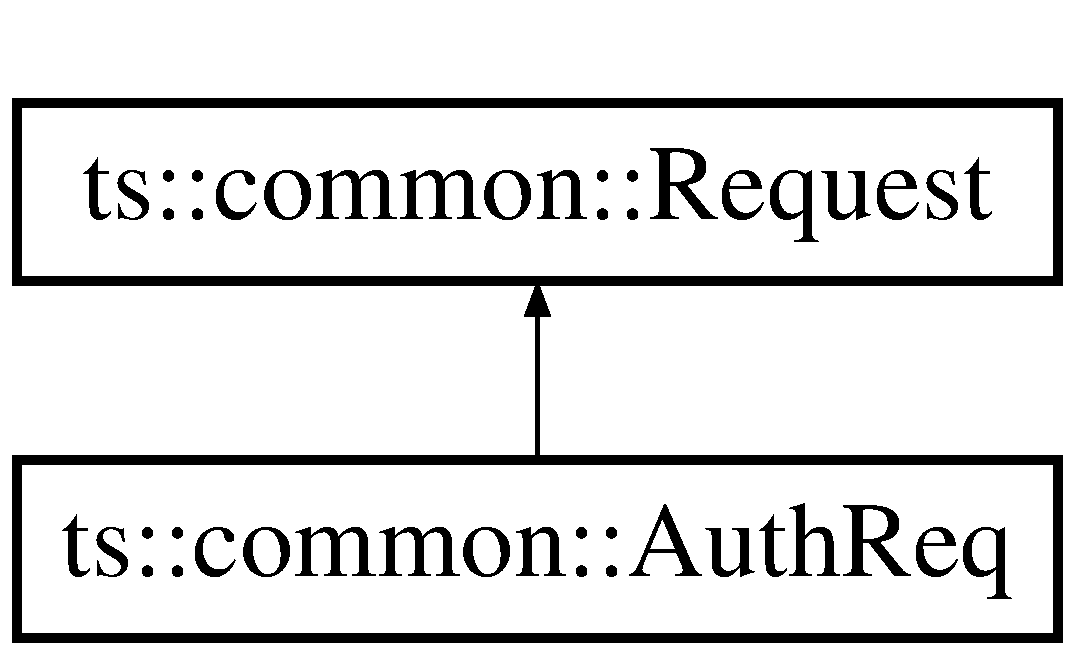
\includegraphics[height=2.000000cm]{structts_1_1common_1_1_auth_req}
\end{center}
\end{figure}
\subsection*{Public Member Functions}
\begin{DoxyCompactItemize}
\item 
\mbox{\Hypertarget{structts_1_1common_1_1_auth_req_a68203d787f55a41a7a9d61c54c27e5f2}\label{structts_1_1common_1_1_auth_req_a68203d787f55a41a7a9d61c54c27e5f2}} 
{\bfseries Auth\+Req} (std\+::string const \&from, std\+::string const \&to, std\+::string const \&pub\+Key=\char`\"{}\char`\"{})
\item 
\mbox{\Hypertarget{structts_1_1common_1_1_auth_req_add23cde2f1b4172b64c00688e7f1b3db}\label{structts_1_1common_1_1_auth_req_add23cde2f1b4172b64c00688e7f1b3db}} 
void {\bfseries from\+Json} (std\+::string const \&json) override
\item 
\mbox{\Hypertarget{structts_1_1common_1_1_auth_req_aafde04d1ffbf65d6789cba70a37320a0}\label{structts_1_1common_1_1_auth_req_aafde04d1ffbf65d6789cba70a37320a0}} 
std\+::string {\bfseries to\+Json} () override
\item 
\mbox{\Hypertarget{structts_1_1common_1_1_auth_req_a0d923334f66a22c644ad04dae909e4dd}\label{structts_1_1common_1_1_auth_req_a0d923334f66a22c644ad04dae909e4dd}} 
int {\bfseries get\+Id} () const override
\end{DoxyCompactItemize}
\subsection*{Public Attributes}
\begin{DoxyCompactItemize}
\item 
\mbox{\Hypertarget{structts_1_1common_1_1_auth_req_a09f27d7320f0eb94cfb1c8bbfec6009b}\label{structts_1_1common_1_1_auth_req_a09f27d7320f0eb94cfb1c8bbfec6009b}} 
std\+::string {\bfseries pub\+Key}
\end{DoxyCompactItemize}
\subsection*{Additional Inherited Members}


The documentation for this struct was generated from the following file\+:\begin{DoxyCompactItemize}
\item 
Request/Auth\+Req.\+hpp\end{DoxyCompactItemize}

\hypertarget{structts_1_1common_1_1_auth_resp}{}\section{ts\+:\+:common\+:\+:Auth\+Resp Struct Reference}
\label{structts_1_1common_1_1_auth_resp}\index{ts\+::common\+::\+Auth\+Resp@{ts\+::common\+::\+Auth\+Resp}}
Inheritance diagram for ts\+:\+:common\+:\+:Auth\+Resp\+:\begin{figure}[H]
\begin{center}
\leavevmode
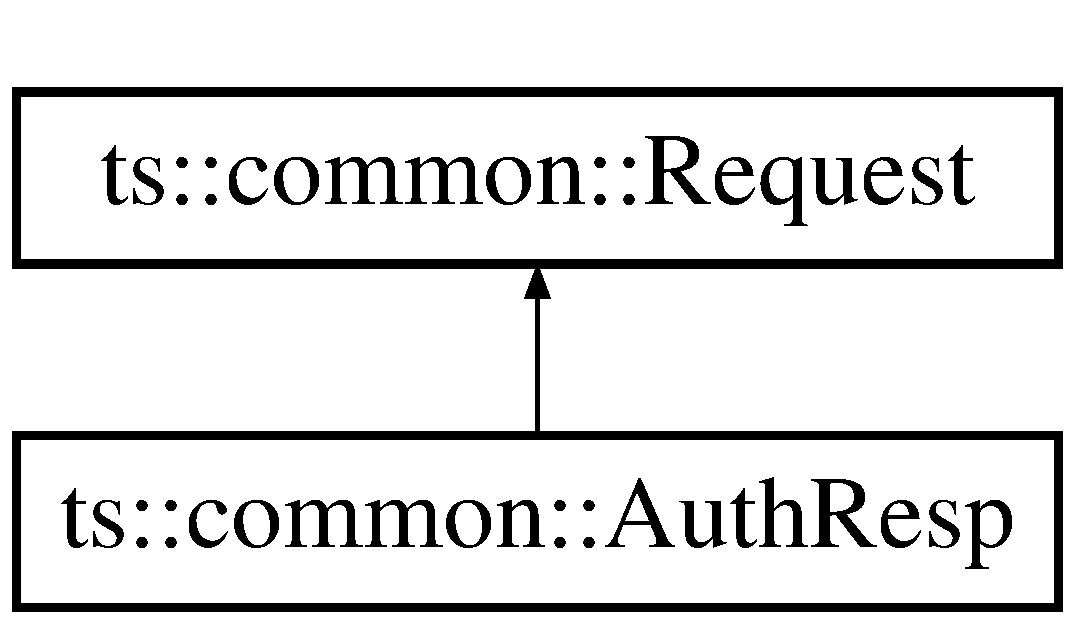
\includegraphics[height=2.000000cm]{structts_1_1common_1_1_auth_resp}
\end{center}
\end{figure}
\subsection*{Public Member Functions}
\begin{DoxyCompactItemize}
\item 
\mbox{\Hypertarget{structts_1_1common_1_1_auth_resp_a6e21274493a765e77ec01e8fc2fb7f50}\label{structts_1_1common_1_1_auth_resp_a6e21274493a765e77ec01e8fc2fb7f50}} 
{\bfseries Auth\+Resp} (std\+::string const \&from, std\+::string const \&to, std\+::string const \&pub\+Key, bool is\+Auth)
\item 
\mbox{\Hypertarget{structts_1_1common_1_1_auth_resp_ad657f20221ab1c81533cabdd7088a951}\label{structts_1_1common_1_1_auth_resp_ad657f20221ab1c81533cabdd7088a951}} 
int {\bfseries get\+Id} () const override
\item 
\mbox{\Hypertarget{structts_1_1common_1_1_auth_resp_a200cf43981dbe5e19d4504f1c9e64faf}\label{structts_1_1common_1_1_auth_resp_a200cf43981dbe5e19d4504f1c9e64faf}} 
std\+::string {\bfseries to\+Json} () override
\end{DoxyCompactItemize}
\subsection*{Public Attributes}
\begin{DoxyCompactItemize}
\item 
\mbox{\Hypertarget{structts_1_1common_1_1_auth_resp_abba0baaf574b6ceb08c8bbe41f9bd122}\label{structts_1_1common_1_1_auth_resp_abba0baaf574b6ceb08c8bbe41f9bd122}} 
std\+::string {\bfseries pub\+Key}
\item 
\mbox{\Hypertarget{structts_1_1common_1_1_auth_resp_a1ce64ac646961e594a16fca9eb596be8}\label{structts_1_1common_1_1_auth_resp_a1ce64ac646961e594a16fca9eb596be8}} 
bool {\bfseries is\+Auth}
\end{DoxyCompactItemize}
\subsection*{Additional Inherited Members}


The documentation for this struct was generated from the following file\+:\begin{DoxyCompactItemize}
\item 
Request/Auth\+Resp.\+hpp\end{DoxyCompactItemize}

\hypertarget{structts_1_1common_1_1_click_activity_req}{}\section{ts\+:\+:common\+:\+:Click\+Activity\+Req Struct Reference}
\label{structts_1_1common_1_1_click_activity_req}\index{ts\+::common\+::\+Click\+Activity\+Req@{ts\+::common\+::\+Click\+Activity\+Req}}
Inheritance diagram for ts\+:\+:common\+:\+:Click\+Activity\+Req\+:\begin{figure}[H]
\begin{center}
\leavevmode
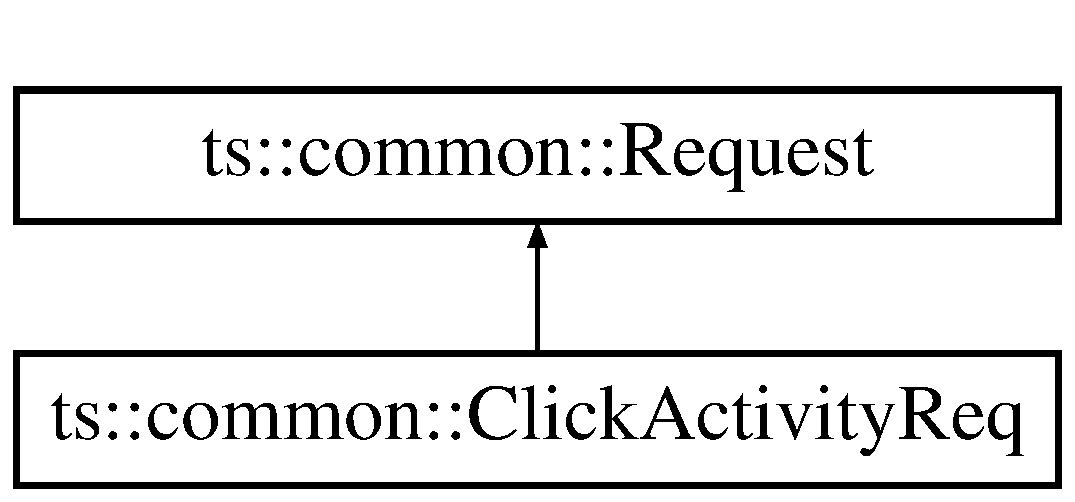
\includegraphics[height=2.000000cm]{structts_1_1common_1_1_click_activity_req}
\end{center}
\end{figure}
\subsection*{Public Member Functions}
\begin{DoxyCompactItemize}
\item 
\mbox{\Hypertarget{structts_1_1common_1_1_click_activity_req_aa5807c63f2ae8390684bdfa493d82116}\label{structts_1_1common_1_1_click_activity_req_aa5807c63f2ae8390684bdfa493d82116}} 
{\bfseries Click\+Activity\+Req} (std\+::string const \&from, std\+::string const \&to, Click\+Type type, int clickX, int clickY)
\item 
\mbox{\Hypertarget{structts_1_1common_1_1_click_activity_req_af6cfec5d4a169be3e72853c7c5ba53a8}\label{structts_1_1common_1_1_click_activity_req_af6cfec5d4a169be3e72853c7c5ba53a8}} 
int {\bfseries get\+Id} () const override
\item 
\mbox{\Hypertarget{structts_1_1common_1_1_click_activity_req_adddea5af0019044379a7dc166a11a25f}\label{structts_1_1common_1_1_click_activity_req_adddea5af0019044379a7dc166a11a25f}} 
void {\bfseries from\+Json} (std\+::string const \&json) override
\item 
\mbox{\Hypertarget{structts_1_1common_1_1_click_activity_req_a67f4c080ad3266f205a7bf1d064c456c}\label{structts_1_1common_1_1_click_activity_req_a67f4c080ad3266f205a7bf1d064c456c}} 
std\+::string {\bfseries to\+Json} () override
\end{DoxyCompactItemize}
\subsection*{Public Attributes}
\begin{DoxyCompactItemize}
\item 
\mbox{\Hypertarget{structts_1_1common_1_1_click_activity_req_addbe8081a2c2f4654dc22247b60a78e4}\label{structts_1_1common_1_1_click_activity_req_addbe8081a2c2f4654dc22247b60a78e4}} 
Click\+Type {\bfseries click\+Type}
\item 
\mbox{\Hypertarget{structts_1_1common_1_1_click_activity_req_a9348fe09e1bd80c0786a4fb109877b76}\label{structts_1_1common_1_1_click_activity_req_a9348fe09e1bd80c0786a4fb109877b76}} 
int {\bfseries clickX}
\item 
\mbox{\Hypertarget{structts_1_1common_1_1_click_activity_req_a60a336ea52f8cd234578c9c29224589e}\label{structts_1_1common_1_1_click_activity_req_a60a336ea52f8cd234578c9c29224589e}} 
int {\bfseries clickY}
\item 
\mbox{\Hypertarget{structts_1_1common_1_1_click_activity_req_ab07ecd544a06dd822ee4be0d98b070af}\label{structts_1_1common_1_1_click_activity_req_ab07ecd544a06dd822ee4be0d98b070af}} 
std\+::string {\bfseries process\+Info}
\end{DoxyCompactItemize}
\subsection*{Additional Inherited Members}


The documentation for this struct was generated from the following file\+:\begin{DoxyCompactItemize}
\item 
Request/Click\+Activity\+Req.\+hpp\end{DoxyCompactItemize}

\hypertarget{classts_1_1_client}{}\section{ts\+:\+:Client Class Reference}
\label{classts_1_1_client}\index{ts\+::\+Client@{ts\+::\+Client}}
Inheritance diagram for ts\+:\+:Client\+:\begin{figure}[H]
\begin{center}
\leavevmode
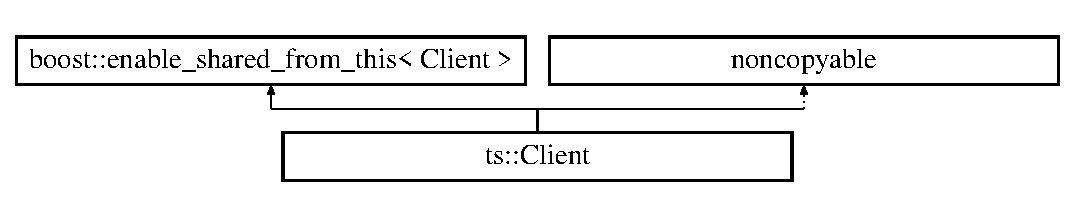
\includegraphics[height=2.000000cm]{classts_1_1_client}
\end{center}
\end{figure}
\subsection*{Public Member Functions}
\begin{DoxyCompactItemize}
\item 
\mbox{\Hypertarget{classts_1_1_client_a892b1cd679659a7b35dc2da44938e509}\label{classts_1_1_client_a892b1cd679659a7b35dc2da44938e509}} 
{\bfseries Client} (boost\+::asio\+::io\+\_\+service \&ios)
\item 
boost\+::asio\+::ip\+::tcp\+::socket \& \hyperlink{classts_1_1_client_a02aaec358cb00665465e5ebb0e031ea2}{get\+Socket} ()
\item 
\mbox{\Hypertarget{classts_1_1_client_a5f37c3c03162add1fcf084cd10bf4d78}\label{classts_1_1_client_a5f37c3c03162add1fcf084cd10bf4d78}} 
void \hyperlink{classts_1_1_client_a5f37c3c03162add1fcf084cd10bf4d78}{start} ()
\begin{DoxyCompactList}\small\item\em Start the client. \end{DoxyCompactList}\item 
\mbox{\Hypertarget{classts_1_1_client_aec10dc278b3e8ede97beee9ef4393076}\label{classts_1_1_client_aec10dc278b3e8ede97beee9ef4393076}} 
void \hyperlink{classts_1_1_client_aec10dc278b3e8ede97beee9ef4393076}{stop} ()
\begin{DoxyCompactList}\small\item\em Stop the client. \end{DoxyCompactList}\item 
void \hyperlink{classts_1_1_client_a524c5585285a81de781fc7e1d1cd3a16}{set\+On\+Stop\+Client\+Callback} (std\+::function$<$ void(boost\+::shared\+\_\+ptr$<$ \hyperlink{classts_1_1_client}{Client} $>$ client)$>$ on\+Stop\+Client)
\item 
void \hyperlink{classts_1_1_client_a60a5793486ab652d476b930dc432884a}{send\+Command} (std\+::string const \&msg)
\item 
std\+::string \hyperlink{classts_1_1_client_a76240db1ee8a0c56be0e7b88e3f7e52e}{get\+Info} ()
\item 
\mbox{\Hypertarget{classts_1_1_client_a3f8170f3d749c048125dc9aaf312c7bf}\label{classts_1_1_client_a3f8170f3d749c048125dc9aaf312c7bf}} 
void \hyperlink{classts_1_1_client_a3f8170f3d749c048125dc9aaf312c7bf}{send\+Server\+Disconnect\+Request} ()
\begin{DoxyCompactList}\small\item\em Send a request to notify server disconnection. \end{DoxyCompactList}\item 
void \hyperlink{classts_1_1_client_a4fd19e3b8dae284cd0f30bf7bd525720}{set\+Data\+Recorder} (std\+::shared\+\_\+ptr$<$ \hyperlink{classts_1_1_i_data_recorder}{I\+Data\+Recorder} $>$ data\+Recorder)
\end{DoxyCompactItemize}
\subsection*{Friends}
\begin{DoxyCompactItemize}
\item 
\mbox{\Hypertarget{classts_1_1_client_a885dbb0d49886f3402b8ed12ab9c076a}\label{classts_1_1_client_a885dbb0d49886f3402b8ed12ab9c076a}} 
class {\bfseries Request\+Handler}
\end{DoxyCompactItemize}


\subsection{Member Function Documentation}
\mbox{\Hypertarget{classts_1_1_client_a76240db1ee8a0c56be0e7b88e3f7e52e}\label{classts_1_1_client_a76240db1ee8a0c56be0e7b88e3f7e52e}} 
\index{ts\+::\+Client@{ts\+::\+Client}!get\+Info@{get\+Info}}
\index{get\+Info@{get\+Info}!ts\+::\+Client@{ts\+::\+Client}}
\subsubsection{\texorpdfstring{get\+Info()}{getInfo()}}
{\footnotesize\ttfamily std\+::string ts\+::\+Client\+::get\+Info (\begin{DoxyParamCaption}{ }\end{DoxyParamCaption})}

Return info about the client \begin{DoxyReturn}{Returns}

\end{DoxyReturn}
\mbox{\Hypertarget{classts_1_1_client_a02aaec358cb00665465e5ebb0e031ea2}\label{classts_1_1_client_a02aaec358cb00665465e5ebb0e031ea2}} 
\index{ts\+::\+Client@{ts\+::\+Client}!get\+Socket@{get\+Socket}}
\index{get\+Socket@{get\+Socket}!ts\+::\+Client@{ts\+::\+Client}}
\subsubsection{\texorpdfstring{get\+Socket()}{getSocket()}}
{\footnotesize\ttfamily boost\+::asio\+::ip\+::tcp\+::socket\& ts\+::\+Client\+::get\+Socket (\begin{DoxyParamCaption}{ }\end{DoxyParamCaption})}

Return the boost socket instance \begin{DoxyReturn}{Returns}

\end{DoxyReturn}
\mbox{\Hypertarget{classts_1_1_client_a60a5793486ab652d476b930dc432884a}\label{classts_1_1_client_a60a5793486ab652d476b930dc432884a}} 
\index{ts\+::\+Client@{ts\+::\+Client}!send\+Command@{send\+Command}}
\index{send\+Command@{send\+Command}!ts\+::\+Client@{ts\+::\+Client}}
\subsubsection{\texorpdfstring{send\+Command()}{sendCommand()}}
{\footnotesize\ttfamily void ts\+::\+Client\+::send\+Command (\begin{DoxyParamCaption}\item[{std\+::string const \&}]{msg }\end{DoxyParamCaption})}

Send command 
\begin{DoxyParams}{Parameters}
{\em msg} & \\
\hline
\end{DoxyParams}
\mbox{\Hypertarget{classts_1_1_client_a4fd19e3b8dae284cd0f30bf7bd525720}\label{classts_1_1_client_a4fd19e3b8dae284cd0f30bf7bd525720}} 
\index{ts\+::\+Client@{ts\+::\+Client}!set\+Data\+Recorder@{set\+Data\+Recorder}}
\index{set\+Data\+Recorder@{set\+Data\+Recorder}!ts\+::\+Client@{ts\+::\+Client}}
\subsubsection{\texorpdfstring{set\+Data\+Recorder()}{setDataRecorder()}}
{\footnotesize\ttfamily void ts\+::\+Client\+::set\+Data\+Recorder (\begin{DoxyParamCaption}\item[{std\+::shared\+\_\+ptr$<$ \hyperlink{classts_1_1_i_data_recorder}{I\+Data\+Recorder} $>$}]{data\+Recorder }\end{DoxyParamCaption})}

Set the data recorder type 
\begin{DoxyParams}{Parameters}
{\em data\+Recorder} & \\
\hline
\end{DoxyParams}
\mbox{\Hypertarget{classts_1_1_client_a524c5585285a81de781fc7e1d1cd3a16}\label{classts_1_1_client_a524c5585285a81de781fc7e1d1cd3a16}} 
\index{ts\+::\+Client@{ts\+::\+Client}!set\+On\+Stop\+Client\+Callback@{set\+On\+Stop\+Client\+Callback}}
\index{set\+On\+Stop\+Client\+Callback@{set\+On\+Stop\+Client\+Callback}!ts\+::\+Client@{ts\+::\+Client}}
\subsubsection{\texorpdfstring{set\+On\+Stop\+Client\+Callback()}{setOnStopClientCallback()}}
{\footnotesize\ttfamily void ts\+::\+Client\+::set\+On\+Stop\+Client\+Callback (\begin{DoxyParamCaption}\item[{std\+::function$<$ void(boost\+::shared\+\_\+ptr$<$ \hyperlink{classts_1_1_client}{Client} $>$ client)$>$}]{on\+Stop\+Client }\end{DoxyParamCaption})}

Set the on stop client callback 
\begin{DoxyParams}{Parameters}
{\em on\+Stop\+Client} & \\
\hline
\end{DoxyParams}


The documentation for this class was generated from the following file\+:\begin{DoxyCompactItemize}
\item 
Client/Client.\+hpp\end{DoxyCompactItemize}

\hypertarget{classts_1_1_client_manager}{}\section{ts\+:\+:Client\+Manager Class Reference}
\label{classts_1_1_client_manager}\index{ts\+::\+Client\+Manager@{ts\+::\+Client\+Manager}}
\subsection*{Public Member Functions}
\begin{DoxyCompactItemize}
\item 
void \hyperlink{classts_1_1_client_manager_a259240643ded77312811f4d4c781c8df}{add} (Client\+Ptr \&client)
\item 
void \hyperlink{classts_1_1_client_manager_a3d622eee3a7d3101d5c77f2dc5f241c2}{remove} (Client\+Ptr \&client)
\item 
void \hyperlink{classts_1_1_client_manager_a1622242546ab02fe20ad844c519cbc0a}{stop} (Client\+Ptr \&client)
\item 
\mbox{\Hypertarget{classts_1_1_client_manager_ab5c1ba814ab730711082ca77bbcfbc97}\label{classts_1_1_client_manager_ab5c1ba814ab730711082ca77bbcfbc97}} 
void \hyperlink{classts_1_1_client_manager_ab5c1ba814ab730711082ca77bbcfbc97}{stop\+All} ()
\begin{DoxyCompactList}\small\item\em Stop all client. \end{DoxyCompactList}\item 
void \hyperlink{classts_1_1_client_manager_a4bf9aa9c7ef6f10ae11a8c3408183ed3}{foreach} (On\+Foreach\+Func on\+Foreach)
\end{DoxyCompactItemize}


\subsection{Member Function Documentation}
\mbox{\Hypertarget{classts_1_1_client_manager_a259240643ded77312811f4d4c781c8df}\label{classts_1_1_client_manager_a259240643ded77312811f4d4c781c8df}} 
\index{ts\+::\+Client\+Manager@{ts\+::\+Client\+Manager}!add@{add}}
\index{add@{add}!ts\+::\+Client\+Manager@{ts\+::\+Client\+Manager}}
\subsubsection{\texorpdfstring{add()}{add()}}
{\footnotesize\ttfamily void ts\+::\+Client\+Manager\+::add (\begin{DoxyParamCaption}\item[{Client\+Ptr \&}]{client }\end{DoxyParamCaption})}

Add new client 
\begin{DoxyParams}{Parameters}
{\em client} & \\
\hline
\end{DoxyParams}
\mbox{\Hypertarget{classts_1_1_client_manager_a4bf9aa9c7ef6f10ae11a8c3408183ed3}\label{classts_1_1_client_manager_a4bf9aa9c7ef6f10ae11a8c3408183ed3}} 
\index{ts\+::\+Client\+Manager@{ts\+::\+Client\+Manager}!foreach@{foreach}}
\index{foreach@{foreach}!ts\+::\+Client\+Manager@{ts\+::\+Client\+Manager}}
\subsubsection{\texorpdfstring{foreach()}{foreach()}}
{\footnotesize\ttfamily void ts\+::\+Client\+Manager\+::foreach (\begin{DoxyParamCaption}\item[{On\+Foreach\+Func}]{on\+Foreach }\end{DoxyParamCaption})}

Apply a function on clients 
\begin{DoxyParams}{Parameters}
{\em on\+Foreach} & \\
\hline
\end{DoxyParams}
\mbox{\Hypertarget{classts_1_1_client_manager_a3d622eee3a7d3101d5c77f2dc5f241c2}\label{classts_1_1_client_manager_a3d622eee3a7d3101d5c77f2dc5f241c2}} 
\index{ts\+::\+Client\+Manager@{ts\+::\+Client\+Manager}!remove@{remove}}
\index{remove@{remove}!ts\+::\+Client\+Manager@{ts\+::\+Client\+Manager}}
\subsubsection{\texorpdfstring{remove()}{remove()}}
{\footnotesize\ttfamily void ts\+::\+Client\+Manager\+::remove (\begin{DoxyParamCaption}\item[{Client\+Ptr \&}]{client }\end{DoxyParamCaption})}

Remove client 
\begin{DoxyParams}{Parameters}
{\em client} & \\
\hline
\end{DoxyParams}
\mbox{\Hypertarget{classts_1_1_client_manager_a1622242546ab02fe20ad844c519cbc0a}\label{classts_1_1_client_manager_a1622242546ab02fe20ad844c519cbc0a}} 
\index{ts\+::\+Client\+Manager@{ts\+::\+Client\+Manager}!stop@{stop}}
\index{stop@{stop}!ts\+::\+Client\+Manager@{ts\+::\+Client\+Manager}}
\subsubsection{\texorpdfstring{stop()}{stop()}}
{\footnotesize\ttfamily void ts\+::\+Client\+Manager\+::stop (\begin{DoxyParamCaption}\item[{Client\+Ptr \&}]{client }\end{DoxyParamCaption})}

Stop a client 
\begin{DoxyParams}{Parameters}
{\em client} & \\
\hline
\end{DoxyParams}


The documentation for this class was generated from the following file\+:\begin{DoxyCompactItemize}
\item 
Client/Client\+Manager.\+hpp\end{DoxyCompactItemize}

\hypertarget{classts_1_1common_1_1tcp_1_1_client_socket}{}\section{ts\+:\+:common\+:\+:tcp\+:\+:Client\+Socket Class Reference}
\label{classts_1_1common_1_1tcp_1_1_client_socket}\index{ts\+::common\+::tcp\+::\+Client\+Socket@{ts\+::common\+::tcp\+::\+Client\+Socket}}
\subsection*{Public Member Functions}
\begin{DoxyCompactItemize}
\item 
\mbox{\Hypertarget{classts_1_1common_1_1tcp_1_1_client_socket_a2d03e028676bd5f58db35c92ebe42029}\label{classts_1_1common_1_1tcp_1_1_client_socket_a2d03e028676bd5f58db35c92ebe42029}} 
{\bfseries Client\+Socket} (boost\+::asio\+::io\+\_\+service \&ios)
\item 
void \hyperlink{classts_1_1common_1_1tcp_1_1_client_socket_a0dda673c5f81c70c398c96a2a11ba152}{connect} (std\+::string const \&host, unsigned short port)
\item 
void \hyperlink{classts_1_1common_1_1tcp_1_1_client_socket_a6e852eb6629afd2fa253ccd3fd8a591a}{async\+Connect} (std\+::string const \&host, unsigned short port, On\+Connect\+Func on\+Connect)
\item 
void \hyperlink{classts_1_1common_1_1tcp_1_1_client_socket_a294447025579635cbfa7fe1829eb15a3}{close} ()
\item 
boost\+::asio\+::ip\+::tcp\+::socket \& \hyperlink{classts_1_1common_1_1tcp_1_1_client_socket_a951aaa6937d4acd0020d30aa8481a485}{get\+Socket} ()
\item 
bool \hyperlink{classts_1_1common_1_1tcp_1_1_client_socket_a654e7f9378b5143032c767486f1752f2}{is\+Connected} () const
\item 
size\+\_\+t \hyperlink{classts_1_1common_1_1tcp_1_1_client_socket_aa408490515485ebc5925685fa4cc4b93}{write} (void const $\ast$data, size\+\_\+t size)
\item 
void \hyperlink{classts_1_1common_1_1tcp_1_1_client_socket_acab3419c27934c50c8020b255af1a3ee}{async\+Write} (void const $\ast$data, size\+\_\+t size, On\+Write\+Func on\+Write=nullptr)
\item 
size\+\_\+t \hyperlink{classts_1_1common_1_1tcp_1_1_client_socket_a7876d2f81c6bf60f628973577dfabd2a}{read} (void $\ast$data, size\+\_\+t size)
\item 
void \hyperlink{classts_1_1common_1_1tcp_1_1_client_socket_afea6b565d0621b6d19648c0259b85e95}{async\+Read} (void $\ast$data, size\+\_\+t size, On\+Read\+Func on\+Read=nullptr)
\item 
void \hyperlink{classts_1_1common_1_1tcp_1_1_client_socket_a0fdc353f373b36eba7096ca88b957842}{set\+On\+Read\+Callback} (On\+Read\+Func on\+Read)
\item 
void \hyperlink{classts_1_1common_1_1tcp_1_1_client_socket_a6dc4758bd4b328dec0ee8cbc1a39820b}{set\+On\+Write\+Callback} (On\+Write\+Func on\+Write)
\item 
void \hyperlink{classts_1_1common_1_1tcp_1_1_client_socket_aeb8c00f0828b0d61c0f2a4b1aa486ff4}{set\+On\+Connect\+Callback} (On\+Connect\+Func on\+Connect)
\item 
\mbox{\Hypertarget{classts_1_1common_1_1tcp_1_1_client_socket_ae03a9e025ffc06eede204954a634a96e}\label{classts_1_1common_1_1tcp_1_1_client_socket_ae03a9e025ffc06eede204954a634a96e}} 
void {\bfseries set\+On\+Disconnect\+Callback} (On\+Disconnect on\+Disconnect)
\item 
std\+::string const  \& \hyperlink{classts_1_1common_1_1tcp_1_1_client_socket_a77d1bdcdd306a6487626ecbbdb4a0910}{get\+Address} ()
\item 
unsigned short \hyperlink{classts_1_1common_1_1tcp_1_1_client_socket_a3e17803779e94e89f3cda035a280d315}{get\+Port} ()
\item 
\mbox{\Hypertarget{classts_1_1common_1_1tcp_1_1_client_socket_a748fcc1565b851f1dd87dcf8c2d63057}\label{classts_1_1common_1_1tcp_1_1_client_socket_a748fcc1565b851f1dd87dcf8c2d63057}} 
void {\bfseries run} ()
\item 
\mbox{\Hypertarget{classts_1_1common_1_1tcp_1_1_client_socket_a7d1a90e4e2f918b899315a68cc3edd55}\label{classts_1_1common_1_1tcp_1_1_client_socket_a7d1a90e4e2f918b899315a68cc3edd55}} 
std\+::string {\bfseries get\+Info} ()
\item 
\mbox{\Hypertarget{classts_1_1common_1_1tcp_1_1_client_socket_aed2b9b1b3d589aaef9476df1f0800a6c}\label{classts_1_1common_1_1tcp_1_1_client_socket_aed2b9b1b3d589aaef9476df1f0800a6c}} 
void {\bfseries force\+Connection\+Status\+Has} (bool i)
\end{DoxyCompactItemize}
\subsection*{Protected Attributes}
\begin{DoxyCompactItemize}
\item 
\mbox{\Hypertarget{classts_1_1common_1_1tcp_1_1_client_socket_acb932dfbb7d1287af95c0f900563d8f7}\label{classts_1_1common_1_1tcp_1_1_client_socket_acb932dfbb7d1287af95c0f900563d8f7}} 
boost\+::asio\+::io\+\_\+service \& {\bfseries m\+Ios}
\item 
\mbox{\Hypertarget{classts_1_1common_1_1tcp_1_1_client_socket_a000d67633711815a8f2dc16acc9d2035}\label{classts_1_1common_1_1tcp_1_1_client_socket_a000d67633711815a8f2dc16acc9d2035}} 
boost\+::asio\+::ip\+::tcp\+::socket {\bfseries m\+Socket}
\item 
\mbox{\Hypertarget{classts_1_1common_1_1tcp_1_1_client_socket_aeede5987e5beb49f60c14840e84fd4eb}\label{classts_1_1common_1_1tcp_1_1_client_socket_aeede5987e5beb49f60c14840e84fd4eb}} 
bool {\bfseries m\+Is\+Connected}
\item 
\mbox{\Hypertarget{classts_1_1common_1_1tcp_1_1_client_socket_a5ebac0ae9230a9659b486d43a8b27b9b}\label{classts_1_1common_1_1tcp_1_1_client_socket_a5ebac0ae9230a9659b486d43a8b27b9b}} 
On\+Write\+Func {\bfseries m\+On\+Write}
\item 
\mbox{\Hypertarget{classts_1_1common_1_1tcp_1_1_client_socket_a116da217aaa9c4b18a6d7eb17994b58d}\label{classts_1_1common_1_1tcp_1_1_client_socket_a116da217aaa9c4b18a6d7eb17994b58d}} 
On\+Read\+Func {\bfseries m\+On\+Read}
\item 
\mbox{\Hypertarget{classts_1_1common_1_1tcp_1_1_client_socket_a79c7916f52cd6b18935200e042d55483}\label{classts_1_1common_1_1tcp_1_1_client_socket_a79c7916f52cd6b18935200e042d55483}} 
On\+Connect\+Func {\bfseries m\+On\+Connect}
\item 
\mbox{\Hypertarget{classts_1_1common_1_1tcp_1_1_client_socket_a3e19605ebf2eac6fe9d1b7c0e2c51fa1}\label{classts_1_1common_1_1tcp_1_1_client_socket_a3e19605ebf2eac6fe9d1b7c0e2c51fa1}} 
On\+Disconnect {\bfseries m\+On\+Disconnect}
\item 
\mbox{\Hypertarget{classts_1_1common_1_1tcp_1_1_client_socket_ad6ce1b1f3dfed87d9498610fcb75a5ef}\label{classts_1_1common_1_1tcp_1_1_client_socket_ad6ce1b1f3dfed87d9498610fcb75a5ef}} 
std\+::string {\bfseries m\+Address}
\item 
\mbox{\Hypertarget{classts_1_1common_1_1tcp_1_1_client_socket_a86914cea89264845b3e6f2b1213f48b5}\label{classts_1_1common_1_1tcp_1_1_client_socket_a86914cea89264845b3e6f2b1213f48b5}} 
unsigned short {\bfseries m\+Port}
\end{DoxyCompactItemize}


\subsection{Member Function Documentation}
\mbox{\Hypertarget{classts_1_1common_1_1tcp_1_1_client_socket_a6e852eb6629afd2fa253ccd3fd8a591a}\label{classts_1_1common_1_1tcp_1_1_client_socket_a6e852eb6629afd2fa253ccd3fd8a591a}} 
\index{ts\+::common\+::tcp\+::\+Client\+Socket@{ts\+::common\+::tcp\+::\+Client\+Socket}!async\+Connect@{async\+Connect}}
\index{async\+Connect@{async\+Connect}!ts\+::common\+::tcp\+::\+Client\+Socket@{ts\+::common\+::tcp\+::\+Client\+Socket}}
\subsubsection{\texorpdfstring{async\+Connect()}{asyncConnect()}}
{\footnotesize\ttfamily void ts\+::common\+::tcp\+::\+Client\+Socket\+::async\+Connect (\begin{DoxyParamCaption}\item[{std\+::string const \&}]{host,  }\item[{unsigned short}]{port,  }\item[{On\+Connect\+Func}]{on\+Connect }\end{DoxyParamCaption})}

Connect the client to the server asynchronously 
\begin{DoxyParams}{Parameters}
{\em host} & \\
\hline
{\em port} & \\
\hline
\end{DoxyParams}
\mbox{\Hypertarget{classts_1_1common_1_1tcp_1_1_client_socket_afea6b565d0621b6d19648c0259b85e95}\label{classts_1_1common_1_1tcp_1_1_client_socket_afea6b565d0621b6d19648c0259b85e95}} 
\index{ts\+::common\+::tcp\+::\+Client\+Socket@{ts\+::common\+::tcp\+::\+Client\+Socket}!async\+Read@{async\+Read}}
\index{async\+Read@{async\+Read}!ts\+::common\+::tcp\+::\+Client\+Socket@{ts\+::common\+::tcp\+::\+Client\+Socket}}
\subsubsection{\texorpdfstring{async\+Read()}{asyncRead()}}
{\footnotesize\ttfamily void ts\+::common\+::tcp\+::\+Client\+Socket\+::async\+Read (\begin{DoxyParamCaption}\item[{void $\ast$}]{data,  }\item[{size\+\_\+t}]{size,  }\item[{On\+Read\+Func}]{on\+Read = {\ttfamily nullptr} }\end{DoxyParamCaption})}

Read data asynchronously 
\begin{DoxyParams}{Parameters}
{\em data} & \\
\hline
{\em size} & \\
\hline
{\em on\+Read} & \\
\hline
\end{DoxyParams}
\mbox{\Hypertarget{classts_1_1common_1_1tcp_1_1_client_socket_acab3419c27934c50c8020b255af1a3ee}\label{classts_1_1common_1_1tcp_1_1_client_socket_acab3419c27934c50c8020b255af1a3ee}} 
\index{ts\+::common\+::tcp\+::\+Client\+Socket@{ts\+::common\+::tcp\+::\+Client\+Socket}!async\+Write@{async\+Write}}
\index{async\+Write@{async\+Write}!ts\+::common\+::tcp\+::\+Client\+Socket@{ts\+::common\+::tcp\+::\+Client\+Socket}}
\subsubsection{\texorpdfstring{async\+Write()}{asyncWrite()}}
{\footnotesize\ttfamily void ts\+::common\+::tcp\+::\+Client\+Socket\+::async\+Write (\begin{DoxyParamCaption}\item[{void const $\ast$}]{data,  }\item[{size\+\_\+t}]{size,  }\item[{On\+Write\+Func}]{on\+Write = {\ttfamily nullptr} }\end{DoxyParamCaption})}

Write data asynchronously 
\begin{DoxyParams}{Parameters}
{\em data} & \\
\hline
{\em size} & \\
\hline
{\em on\+Write} & \\
\hline
\end{DoxyParams}
\mbox{\Hypertarget{classts_1_1common_1_1tcp_1_1_client_socket_a294447025579635cbfa7fe1829eb15a3}\label{classts_1_1common_1_1tcp_1_1_client_socket_a294447025579635cbfa7fe1829eb15a3}} 
\index{ts\+::common\+::tcp\+::\+Client\+Socket@{ts\+::common\+::tcp\+::\+Client\+Socket}!close@{close}}
\index{close@{close}!ts\+::common\+::tcp\+::\+Client\+Socket@{ts\+::common\+::tcp\+::\+Client\+Socket}}
\subsubsection{\texorpdfstring{close()}{close()}}
{\footnotesize\ttfamily void ts\+::common\+::tcp\+::\+Client\+Socket\+::close (\begin{DoxyParamCaption}{ }\end{DoxyParamCaption})}

Close the Client connection \mbox{\Hypertarget{classts_1_1common_1_1tcp_1_1_client_socket_a0dda673c5f81c70c398c96a2a11ba152}\label{classts_1_1common_1_1tcp_1_1_client_socket_a0dda673c5f81c70c398c96a2a11ba152}} 
\index{ts\+::common\+::tcp\+::\+Client\+Socket@{ts\+::common\+::tcp\+::\+Client\+Socket}!connect@{connect}}
\index{connect@{connect}!ts\+::common\+::tcp\+::\+Client\+Socket@{ts\+::common\+::tcp\+::\+Client\+Socket}}
\subsubsection{\texorpdfstring{connect()}{connect()}}
{\footnotesize\ttfamily void ts\+::common\+::tcp\+::\+Client\+Socket\+::connect (\begin{DoxyParamCaption}\item[{std\+::string const \&}]{host,  }\item[{unsigned short}]{port }\end{DoxyParamCaption})}

Connect the client to the server 
\begin{DoxyParams}{Parameters}
{\em host} & \\
\hline
{\em port} & \\
\hline
\end{DoxyParams}
\mbox{\Hypertarget{classts_1_1common_1_1tcp_1_1_client_socket_a77d1bdcdd306a6487626ecbbdb4a0910}\label{classts_1_1common_1_1tcp_1_1_client_socket_a77d1bdcdd306a6487626ecbbdb4a0910}} 
\index{ts\+::common\+::tcp\+::\+Client\+Socket@{ts\+::common\+::tcp\+::\+Client\+Socket}!get\+Address@{get\+Address}}
\index{get\+Address@{get\+Address}!ts\+::common\+::tcp\+::\+Client\+Socket@{ts\+::common\+::tcp\+::\+Client\+Socket}}
\subsubsection{\texorpdfstring{get\+Address()}{getAddress()}}
{\footnotesize\ttfamily std\+::string const\& ts\+::common\+::tcp\+::\+Client\+Socket\+::get\+Address (\begin{DoxyParamCaption}{ }\end{DoxyParamCaption})}

Return the address \begin{DoxyReturn}{Returns}

\end{DoxyReturn}
\mbox{\Hypertarget{classts_1_1common_1_1tcp_1_1_client_socket_a3e17803779e94e89f3cda035a280d315}\label{classts_1_1common_1_1tcp_1_1_client_socket_a3e17803779e94e89f3cda035a280d315}} 
\index{ts\+::common\+::tcp\+::\+Client\+Socket@{ts\+::common\+::tcp\+::\+Client\+Socket}!get\+Port@{get\+Port}}
\index{get\+Port@{get\+Port}!ts\+::common\+::tcp\+::\+Client\+Socket@{ts\+::common\+::tcp\+::\+Client\+Socket}}
\subsubsection{\texorpdfstring{get\+Port()}{getPort()}}
{\footnotesize\ttfamily unsigned short ts\+::common\+::tcp\+::\+Client\+Socket\+::get\+Port (\begin{DoxyParamCaption}{ }\end{DoxyParamCaption})}

Return the port \begin{DoxyReturn}{Returns}

\end{DoxyReturn}
\mbox{\Hypertarget{classts_1_1common_1_1tcp_1_1_client_socket_a951aaa6937d4acd0020d30aa8481a485}\label{classts_1_1common_1_1tcp_1_1_client_socket_a951aaa6937d4acd0020d30aa8481a485}} 
\index{ts\+::common\+::tcp\+::\+Client\+Socket@{ts\+::common\+::tcp\+::\+Client\+Socket}!get\+Socket@{get\+Socket}}
\index{get\+Socket@{get\+Socket}!ts\+::common\+::tcp\+::\+Client\+Socket@{ts\+::common\+::tcp\+::\+Client\+Socket}}
\subsubsection{\texorpdfstring{get\+Socket()}{getSocket()}}
{\footnotesize\ttfamily boost\+::asio\+::ip\+::tcp\+::socket\& ts\+::common\+::tcp\+::\+Client\+Socket\+::get\+Socket (\begin{DoxyParamCaption}{ }\end{DoxyParamCaption})}

Return the Boost asio socket \begin{DoxyReturn}{Returns}

\end{DoxyReturn}
\mbox{\Hypertarget{classts_1_1common_1_1tcp_1_1_client_socket_a654e7f9378b5143032c767486f1752f2}\label{classts_1_1common_1_1tcp_1_1_client_socket_a654e7f9378b5143032c767486f1752f2}} 
\index{ts\+::common\+::tcp\+::\+Client\+Socket@{ts\+::common\+::tcp\+::\+Client\+Socket}!is\+Connected@{is\+Connected}}
\index{is\+Connected@{is\+Connected}!ts\+::common\+::tcp\+::\+Client\+Socket@{ts\+::common\+::tcp\+::\+Client\+Socket}}
\subsubsection{\texorpdfstring{is\+Connected()}{isConnected()}}
{\footnotesize\ttfamily bool ts\+::common\+::tcp\+::\+Client\+Socket\+::is\+Connected (\begin{DoxyParamCaption}{ }\end{DoxyParamCaption}) const}

Check if the client is connect the server \begin{DoxyReturn}{Returns}

\end{DoxyReturn}
\mbox{\Hypertarget{classts_1_1common_1_1tcp_1_1_client_socket_a7876d2f81c6bf60f628973577dfabd2a}\label{classts_1_1common_1_1tcp_1_1_client_socket_a7876d2f81c6bf60f628973577dfabd2a}} 
\index{ts\+::common\+::tcp\+::\+Client\+Socket@{ts\+::common\+::tcp\+::\+Client\+Socket}!read@{read}}
\index{read@{read}!ts\+::common\+::tcp\+::\+Client\+Socket@{ts\+::common\+::tcp\+::\+Client\+Socket}}
\subsubsection{\texorpdfstring{read()}{read()}}
{\footnotesize\ttfamily size\+\_\+t ts\+::common\+::tcp\+::\+Client\+Socket\+::read (\begin{DoxyParamCaption}\item[{void $\ast$}]{data,  }\item[{size\+\_\+t}]{size }\end{DoxyParamCaption})}

Read data 
\begin{DoxyParams}{Parameters}
{\em data} & \\
\hline
{\em size} & \\
\hline
\end{DoxyParams}
\begin{DoxyReturn}{Returns}

\end{DoxyReturn}
\mbox{\Hypertarget{classts_1_1common_1_1tcp_1_1_client_socket_aeb8c00f0828b0d61c0f2a4b1aa486ff4}\label{classts_1_1common_1_1tcp_1_1_client_socket_aeb8c00f0828b0d61c0f2a4b1aa486ff4}} 
\index{ts\+::common\+::tcp\+::\+Client\+Socket@{ts\+::common\+::tcp\+::\+Client\+Socket}!set\+On\+Connect\+Callback@{set\+On\+Connect\+Callback}}
\index{set\+On\+Connect\+Callback@{set\+On\+Connect\+Callback}!ts\+::common\+::tcp\+::\+Client\+Socket@{ts\+::common\+::tcp\+::\+Client\+Socket}}
\subsubsection{\texorpdfstring{set\+On\+Connect\+Callback()}{setOnConnectCallback()}}
{\footnotesize\ttfamily void ts\+::common\+::tcp\+::\+Client\+Socket\+::set\+On\+Connect\+Callback (\begin{DoxyParamCaption}\item[{On\+Connect\+Func}]{on\+Connect }\end{DoxyParamCaption})}

Set the callback for async\+Connect \begin{DoxySeeAlso}{See also}
\hyperlink{classts_1_1common_1_1tcp_1_1_client_socket_a6e852eb6629afd2fa253ccd3fd8a591a}{async\+Connect} 
\end{DoxySeeAlso}

\begin{DoxyParams}{Parameters}
{\em on\+Connect} & \\
\hline
\end{DoxyParams}
\mbox{\Hypertarget{classts_1_1common_1_1tcp_1_1_client_socket_a0fdc353f373b36eba7096ca88b957842}\label{classts_1_1common_1_1tcp_1_1_client_socket_a0fdc353f373b36eba7096ca88b957842}} 
\index{ts\+::common\+::tcp\+::\+Client\+Socket@{ts\+::common\+::tcp\+::\+Client\+Socket}!set\+On\+Read\+Callback@{set\+On\+Read\+Callback}}
\index{set\+On\+Read\+Callback@{set\+On\+Read\+Callback}!ts\+::common\+::tcp\+::\+Client\+Socket@{ts\+::common\+::tcp\+::\+Client\+Socket}}
\subsubsection{\texorpdfstring{set\+On\+Read\+Callback()}{setOnReadCallback()}}
{\footnotesize\ttfamily void ts\+::common\+::tcp\+::\+Client\+Socket\+::set\+On\+Read\+Callback (\begin{DoxyParamCaption}\item[{On\+Read\+Func}]{on\+Read }\end{DoxyParamCaption})}

Set the callback for async\+Read \begin{DoxySeeAlso}{See also}
\hyperlink{classts_1_1common_1_1tcp_1_1_client_socket_afea6b565d0621b6d19648c0259b85e95}{async\+Read} 
\end{DoxySeeAlso}

\begin{DoxyParams}{Parameters}
{\em on\+Read} & \\
\hline
\end{DoxyParams}
\mbox{\Hypertarget{classts_1_1common_1_1tcp_1_1_client_socket_a6dc4758bd4b328dec0ee8cbc1a39820b}\label{classts_1_1common_1_1tcp_1_1_client_socket_a6dc4758bd4b328dec0ee8cbc1a39820b}} 
\index{ts\+::common\+::tcp\+::\+Client\+Socket@{ts\+::common\+::tcp\+::\+Client\+Socket}!set\+On\+Write\+Callback@{set\+On\+Write\+Callback}}
\index{set\+On\+Write\+Callback@{set\+On\+Write\+Callback}!ts\+::common\+::tcp\+::\+Client\+Socket@{ts\+::common\+::tcp\+::\+Client\+Socket}}
\subsubsection{\texorpdfstring{set\+On\+Write\+Callback()}{setOnWriteCallback()}}
{\footnotesize\ttfamily void ts\+::common\+::tcp\+::\+Client\+Socket\+::set\+On\+Write\+Callback (\begin{DoxyParamCaption}\item[{On\+Write\+Func}]{on\+Write }\end{DoxyParamCaption})}

Set the callback for async\+Write \begin{DoxySeeAlso}{See also}
\hyperlink{classts_1_1common_1_1tcp_1_1_client_socket_acab3419c27934c50c8020b255af1a3ee}{async\+Write} 
\end{DoxySeeAlso}

\begin{DoxyParams}{Parameters}
{\em on\+Write} & \\
\hline
\end{DoxyParams}
\mbox{\Hypertarget{classts_1_1common_1_1tcp_1_1_client_socket_aa408490515485ebc5925685fa4cc4b93}\label{classts_1_1common_1_1tcp_1_1_client_socket_aa408490515485ebc5925685fa4cc4b93}} 
\index{ts\+::common\+::tcp\+::\+Client\+Socket@{ts\+::common\+::tcp\+::\+Client\+Socket}!write@{write}}
\index{write@{write}!ts\+::common\+::tcp\+::\+Client\+Socket@{ts\+::common\+::tcp\+::\+Client\+Socket}}
\subsubsection{\texorpdfstring{write()}{write()}}
{\footnotesize\ttfamily size\+\_\+t ts\+::common\+::tcp\+::\+Client\+Socket\+::write (\begin{DoxyParamCaption}\item[{void const $\ast$}]{data,  }\item[{size\+\_\+t}]{size }\end{DoxyParamCaption})}

Write data 
\begin{DoxyParams}{Parameters}
{\em data} & \\
\hline
{\em size} & \\
\hline
\end{DoxyParams}
\begin{DoxyReturn}{Returns}

\end{DoxyReturn}


The documentation for this class was generated from the following file\+:\begin{DoxyCompactItemize}
\item 
Socket/Tcp\+Client\+Socket.\+hpp\end{DoxyCompactItemize}

\hypertarget{classts_1_1common_1_1udp_1_1_client_socket}{}\section{ts\+:\+:common\+:\+:udp\+:\+:Client\+Socket Class Reference}
\label{classts_1_1common_1_1udp_1_1_client_socket}\index{ts\+::common\+::udp\+::\+Client\+Socket@{ts\+::common\+::udp\+::\+Client\+Socket}}
Inheritance diagram for ts\+:\+:common\+:\+:udp\+:\+:Client\+Socket\+:\begin{figure}[H]
\begin{center}
\leavevmode
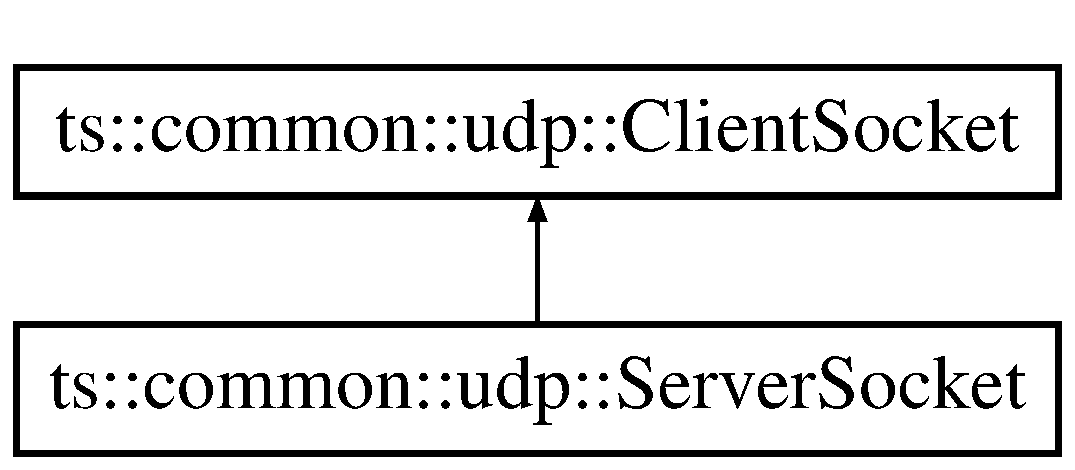
\includegraphics[height=2.000000cm]{classts_1_1common_1_1udp_1_1_client_socket}
\end{center}
\end{figure}
\subsection*{Public Member Functions}
\begin{DoxyCompactItemize}
\item 
\mbox{\Hypertarget{classts_1_1common_1_1udp_1_1_client_socket_a74c773d6063b088437294998da8e7bb3}\label{classts_1_1common_1_1udp_1_1_client_socket_a74c773d6063b088437294998da8e7bb3}} 
{\bfseries Client\+Socket} (boost\+::asio\+::io\+\_\+service \&ios)
\item 
void \hyperlink{classts_1_1common_1_1udp_1_1_client_socket_ad58682dc83e4de4814efe73b7c3f8a03}{close} ()
\item 
boost\+::asio\+::ip\+::udp\+::socket \& \hyperlink{classts_1_1common_1_1udp_1_1_client_socket_a6e7a4527ef58ebb10da1dc456d6ef3d2}{get\+Socket} ()
\item 
size\+\_\+t \hyperlink{classts_1_1common_1_1udp_1_1_client_socket_a21b35f111813fe20dcd40f40c12c0f29}{send\+To} (const std\+::string \&host, unsigned short port, void const $\ast$data, size\+\_\+t size)
\item 
void \hyperlink{classts_1_1common_1_1udp_1_1_client_socket_abe684b5395930b9e46cf1bd3cb8a9c32}{async\+Send\+To} (const std\+::string \&host, unsigned short port, void const $\ast$data, size\+\_\+t size, On\+Send\+To\+Func on\+Send\+To=nullptr)
\item 
size\+\_\+t \hyperlink{classts_1_1common_1_1udp_1_1_client_socket_aebfe2f18331fbb67156c0d2ca479a0de}{receive\+From} (const std\+::string \&host, unsigned short port, void $\ast$data, size\+\_\+t size)
\item 
void \hyperlink{classts_1_1common_1_1udp_1_1_client_socket_ae2789434073141d578f5fd740eb42068}{async\+Receive\+From} (const std\+::string \&host, unsigned short port, void $\ast$data, size\+\_\+t size, On\+Receive\+From\+Func on\+Receive\+From=nullptr)
\item 
void \hyperlink{classts_1_1common_1_1udp_1_1_client_socket_a09aac85aca0ed8908e37d2b189ba6fc9}{set\+On\+Receive\+From\+Callback} (On\+Receive\+From\+Func on\+Receive\+From)
\item 
void \hyperlink{classts_1_1common_1_1udp_1_1_client_socket_a04b10fcde4fa312582b02284a5dbdf6c}{set\+On\+Send\+To\+Callback} (On\+Send\+To\+Func on\+Send\+To)
\item 
std\+::string \hyperlink{classts_1_1common_1_1udp_1_1_client_socket_a812b9a0b3cd680dcc37bd708e46a4329}{get\+Address} () const
\end{DoxyCompactItemize}
\subsection*{Protected Attributes}
\begin{DoxyCompactItemize}
\item 
\mbox{\Hypertarget{classts_1_1common_1_1udp_1_1_client_socket_a60a04fec1d4d4f1be81bfb0a62539c07}\label{classts_1_1common_1_1udp_1_1_client_socket_a60a04fec1d4d4f1be81bfb0a62539c07}} 
boost\+::asio\+::io\+\_\+service \& {\bfseries m\+Ios}
\item 
\mbox{\Hypertarget{classts_1_1common_1_1udp_1_1_client_socket_a7216f8d5c2346cb22cceb64371fe26f3}\label{classts_1_1common_1_1udp_1_1_client_socket_a7216f8d5c2346cb22cceb64371fe26f3}} 
boost\+::asio\+::ip\+::udp\+::socket {\bfseries m\+Socket}
\item 
\mbox{\Hypertarget{classts_1_1common_1_1udp_1_1_client_socket_aad7a08fec800008fd1e6602943ddfc8c}\label{classts_1_1common_1_1udp_1_1_client_socket_aad7a08fec800008fd1e6602943ddfc8c}} 
On\+Send\+To\+Func {\bfseries m\+On\+Send\+To}
\item 
\mbox{\Hypertarget{classts_1_1common_1_1udp_1_1_client_socket_add732d15aa6129e1960e4e5addbe03a3}\label{classts_1_1common_1_1udp_1_1_client_socket_add732d15aa6129e1960e4e5addbe03a3}} 
On\+Receive\+From\+Func {\bfseries m\+On\+Receive\+From}
\end{DoxyCompactItemize}


\subsection{Member Function Documentation}
\mbox{\Hypertarget{classts_1_1common_1_1udp_1_1_client_socket_ae2789434073141d578f5fd740eb42068}\label{classts_1_1common_1_1udp_1_1_client_socket_ae2789434073141d578f5fd740eb42068}} 
\index{ts\+::common\+::udp\+::\+Client\+Socket@{ts\+::common\+::udp\+::\+Client\+Socket}!async\+Receive\+From@{async\+Receive\+From}}
\index{async\+Receive\+From@{async\+Receive\+From}!ts\+::common\+::udp\+::\+Client\+Socket@{ts\+::common\+::udp\+::\+Client\+Socket}}
\subsubsection{\texorpdfstring{async\+Receive\+From()}{asyncReceiveFrom()}}
{\footnotesize\ttfamily void ts\+::common\+::udp\+::\+Client\+Socket\+::async\+Receive\+From (\begin{DoxyParamCaption}\item[{const std\+::string \&}]{host,  }\item[{unsigned short}]{port,  }\item[{void $\ast$}]{data,  }\item[{size\+\_\+t}]{size,  }\item[{On\+Receive\+From\+Func}]{on\+Receive\+From = {\ttfamily nullptr} }\end{DoxyParamCaption})}

receive data asynchronously 
\begin{DoxyParams}{Parameters}
{\em host} & \\
\hline
{\em port} & \\
\hline
{\em data} & \\
\hline
{\em size} & \\
\hline
{\em on\+Receive\+From} & \\
\hline
\end{DoxyParams}
\mbox{\Hypertarget{classts_1_1common_1_1udp_1_1_client_socket_abe684b5395930b9e46cf1bd3cb8a9c32}\label{classts_1_1common_1_1udp_1_1_client_socket_abe684b5395930b9e46cf1bd3cb8a9c32}} 
\index{ts\+::common\+::udp\+::\+Client\+Socket@{ts\+::common\+::udp\+::\+Client\+Socket}!async\+Send\+To@{async\+Send\+To}}
\index{async\+Send\+To@{async\+Send\+To}!ts\+::common\+::udp\+::\+Client\+Socket@{ts\+::common\+::udp\+::\+Client\+Socket}}
\subsubsection{\texorpdfstring{async\+Send\+To()}{asyncSendTo()}}
{\footnotesize\ttfamily void ts\+::common\+::udp\+::\+Client\+Socket\+::async\+Send\+To (\begin{DoxyParamCaption}\item[{const std\+::string \&}]{host,  }\item[{unsigned short}]{port,  }\item[{void const $\ast$}]{data,  }\item[{size\+\_\+t}]{size,  }\item[{On\+Send\+To\+Func}]{on\+Send\+To = {\ttfamily nullptr} }\end{DoxyParamCaption})}

send data asynchronously 
\begin{DoxyParams}{Parameters}
{\em data} & \\
\hline
{\em size} & \\
\hline
{\em on\+Write} & \\
\hline
\end{DoxyParams}
\mbox{\Hypertarget{classts_1_1common_1_1udp_1_1_client_socket_ad58682dc83e4de4814efe73b7c3f8a03}\label{classts_1_1common_1_1udp_1_1_client_socket_ad58682dc83e4de4814efe73b7c3f8a03}} 
\index{ts\+::common\+::udp\+::\+Client\+Socket@{ts\+::common\+::udp\+::\+Client\+Socket}!close@{close}}
\index{close@{close}!ts\+::common\+::udp\+::\+Client\+Socket@{ts\+::common\+::udp\+::\+Client\+Socket}}
\subsubsection{\texorpdfstring{close()}{close()}}
{\footnotesize\ttfamily void ts\+::common\+::udp\+::\+Client\+Socket\+::close (\begin{DoxyParamCaption}{ }\end{DoxyParamCaption})}

Close the \hyperlink{classts_1_1_client}{Client} connection \mbox{\Hypertarget{classts_1_1common_1_1udp_1_1_client_socket_a812b9a0b3cd680dcc37bd708e46a4329}\label{classts_1_1common_1_1udp_1_1_client_socket_a812b9a0b3cd680dcc37bd708e46a4329}} 
\index{ts\+::common\+::udp\+::\+Client\+Socket@{ts\+::common\+::udp\+::\+Client\+Socket}!get\+Address@{get\+Address}}
\index{get\+Address@{get\+Address}!ts\+::common\+::udp\+::\+Client\+Socket@{ts\+::common\+::udp\+::\+Client\+Socket}}
\subsubsection{\texorpdfstring{get\+Address()}{getAddress()}}
{\footnotesize\ttfamily std\+::string ts\+::common\+::udp\+::\+Client\+Socket\+::get\+Address (\begin{DoxyParamCaption}{ }\end{DoxyParamCaption}) const}

Return the address \begin{DoxyReturn}{Returns}

\end{DoxyReturn}
\mbox{\Hypertarget{classts_1_1common_1_1udp_1_1_client_socket_a6e7a4527ef58ebb10da1dc456d6ef3d2}\label{classts_1_1common_1_1udp_1_1_client_socket_a6e7a4527ef58ebb10da1dc456d6ef3d2}} 
\index{ts\+::common\+::udp\+::\+Client\+Socket@{ts\+::common\+::udp\+::\+Client\+Socket}!get\+Socket@{get\+Socket}}
\index{get\+Socket@{get\+Socket}!ts\+::common\+::udp\+::\+Client\+Socket@{ts\+::common\+::udp\+::\+Client\+Socket}}
\subsubsection{\texorpdfstring{get\+Socket()}{getSocket()}}
{\footnotesize\ttfamily boost\+::asio\+::ip\+::udp\+::socket\& ts\+::common\+::udp\+::\+Client\+Socket\+::get\+Socket (\begin{DoxyParamCaption}{ }\end{DoxyParamCaption})}

Return the Boost asio socket \begin{DoxyReturn}{Returns}

\end{DoxyReturn}
\mbox{\Hypertarget{classts_1_1common_1_1udp_1_1_client_socket_aebfe2f18331fbb67156c0d2ca479a0de}\label{classts_1_1common_1_1udp_1_1_client_socket_aebfe2f18331fbb67156c0d2ca479a0de}} 
\index{ts\+::common\+::udp\+::\+Client\+Socket@{ts\+::common\+::udp\+::\+Client\+Socket}!receive\+From@{receive\+From}}
\index{receive\+From@{receive\+From}!ts\+::common\+::udp\+::\+Client\+Socket@{ts\+::common\+::udp\+::\+Client\+Socket}}
\subsubsection{\texorpdfstring{receive\+From()}{receiveFrom()}}
{\footnotesize\ttfamily size\+\_\+t ts\+::common\+::udp\+::\+Client\+Socket\+::receive\+From (\begin{DoxyParamCaption}\item[{const std\+::string \&}]{host,  }\item[{unsigned short}]{port,  }\item[{void $\ast$}]{data,  }\item[{size\+\_\+t}]{size }\end{DoxyParamCaption})}

receive data 
\begin{DoxyParams}{Parameters}
{\em data} & \\
\hline
{\em size} & \\
\hline
\end{DoxyParams}
\begin{DoxyReturn}{Returns}

\end{DoxyReturn}
\mbox{\Hypertarget{classts_1_1common_1_1udp_1_1_client_socket_a21b35f111813fe20dcd40f40c12c0f29}\label{classts_1_1common_1_1udp_1_1_client_socket_a21b35f111813fe20dcd40f40c12c0f29}} 
\index{ts\+::common\+::udp\+::\+Client\+Socket@{ts\+::common\+::udp\+::\+Client\+Socket}!send\+To@{send\+To}}
\index{send\+To@{send\+To}!ts\+::common\+::udp\+::\+Client\+Socket@{ts\+::common\+::udp\+::\+Client\+Socket}}
\subsubsection{\texorpdfstring{send\+To()}{sendTo()}}
{\footnotesize\ttfamily size\+\_\+t ts\+::common\+::udp\+::\+Client\+Socket\+::send\+To (\begin{DoxyParamCaption}\item[{const std\+::string \&}]{host,  }\item[{unsigned short}]{port,  }\item[{void const $\ast$}]{data,  }\item[{size\+\_\+t}]{size }\end{DoxyParamCaption})}

Send data 
\begin{DoxyParams}{Parameters}
{\em host} & \\
\hline
{\em port} & \\
\hline
{\em data} & \\
\hline
{\em size} & \\
\hline
\end{DoxyParams}
\begin{DoxyReturn}{Returns}

\end{DoxyReturn}
\mbox{\Hypertarget{classts_1_1common_1_1udp_1_1_client_socket_a09aac85aca0ed8908e37d2b189ba6fc9}\label{classts_1_1common_1_1udp_1_1_client_socket_a09aac85aca0ed8908e37d2b189ba6fc9}} 
\index{ts\+::common\+::udp\+::\+Client\+Socket@{ts\+::common\+::udp\+::\+Client\+Socket}!set\+On\+Receive\+From\+Callback@{set\+On\+Receive\+From\+Callback}}
\index{set\+On\+Receive\+From\+Callback@{set\+On\+Receive\+From\+Callback}!ts\+::common\+::udp\+::\+Client\+Socket@{ts\+::common\+::udp\+::\+Client\+Socket}}
\subsubsection{\texorpdfstring{set\+On\+Receive\+From\+Callback()}{setOnReceiveFromCallback()}}
{\footnotesize\ttfamily void ts\+::common\+::udp\+::\+Client\+Socket\+::set\+On\+Receive\+From\+Callback (\begin{DoxyParamCaption}\item[{On\+Receive\+From\+Func}]{on\+Receive\+From }\end{DoxyParamCaption})}

Set the callback for async\+Receive\+From \begin{DoxySeeAlso}{See also}
\hyperlink{classts_1_1common_1_1udp_1_1_client_socket_ae2789434073141d578f5fd740eb42068}{async\+Receive\+From} 
\end{DoxySeeAlso}

\begin{DoxyParams}{Parameters}
{\em on\+Receive\+From} & \\
\hline
\end{DoxyParams}
\mbox{\Hypertarget{classts_1_1common_1_1udp_1_1_client_socket_a04b10fcde4fa312582b02284a5dbdf6c}\label{classts_1_1common_1_1udp_1_1_client_socket_a04b10fcde4fa312582b02284a5dbdf6c}} 
\index{ts\+::common\+::udp\+::\+Client\+Socket@{ts\+::common\+::udp\+::\+Client\+Socket}!set\+On\+Send\+To\+Callback@{set\+On\+Send\+To\+Callback}}
\index{set\+On\+Send\+To\+Callback@{set\+On\+Send\+To\+Callback}!ts\+::common\+::udp\+::\+Client\+Socket@{ts\+::common\+::udp\+::\+Client\+Socket}}
\subsubsection{\texorpdfstring{set\+On\+Send\+To\+Callback()}{setOnSendToCallback()}}
{\footnotesize\ttfamily void ts\+::common\+::udp\+::\+Client\+Socket\+::set\+On\+Send\+To\+Callback (\begin{DoxyParamCaption}\item[{On\+Send\+To\+Func}]{on\+Send\+To }\end{DoxyParamCaption})}

Set the callback for async\+Send\+To \begin{DoxySeeAlso}{See also}
\hyperlink{classts_1_1common_1_1udp_1_1_client_socket_abe684b5395930b9e46cf1bd3cb8a9c32}{async\+Send\+To} 
\end{DoxySeeAlso}

\begin{DoxyParams}{Parameters}
{\em on\+Receive\+From} & \\
\hline
\end{DoxyParams}


The documentation for this class was generated from the following file\+:\begin{DoxyCompactItemize}
\item 
Socket/Udp\+Client\+Socket.\+hpp\end{DoxyCompactItemize}

\hypertarget{structts_1_1common_1_1_command_req}{}\section{ts\+:\+:common\+:\+:Command\+Req Struct Reference}
\label{structts_1_1common_1_1_command_req}\index{ts\+::common\+::\+Command\+Req@{ts\+::common\+::\+Command\+Req}}
Inheritance diagram for ts\+:\+:common\+:\+:Command\+Req\+:\begin{figure}[H]
\begin{center}
\leavevmode
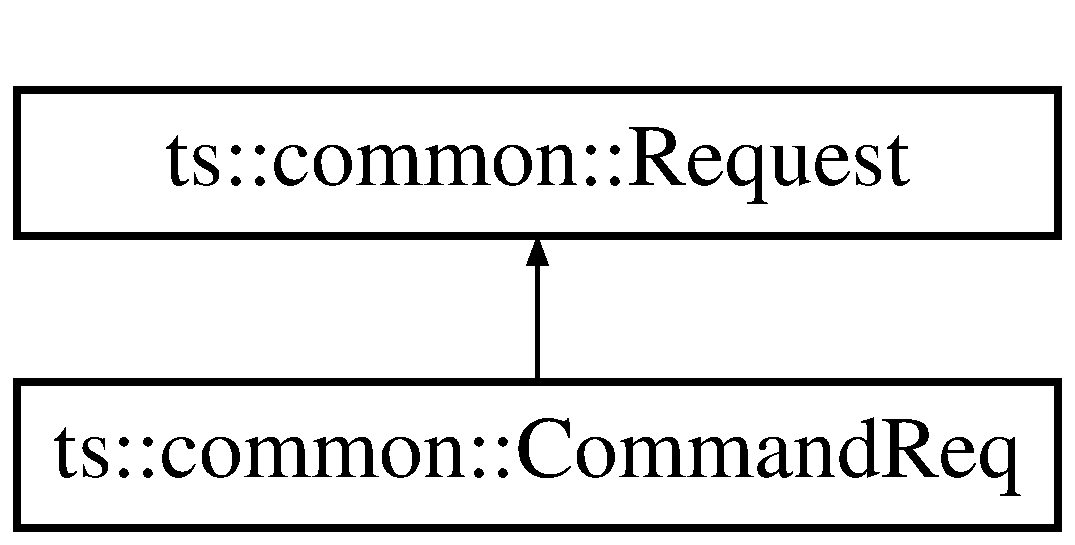
\includegraphics[height=2.000000cm]{structts_1_1common_1_1_command_req}
\end{center}
\end{figure}
\subsection*{Public Member Functions}
\begin{DoxyCompactItemize}
\item 
\mbox{\Hypertarget{structts_1_1common_1_1_command_req_a59cae0eb1c1c91d65f87758c2c0dc6a0}\label{structts_1_1common_1_1_command_req_a59cae0eb1c1c91d65f87758c2c0dc6a0}} 
{\bfseries Command\+Req} (std\+::string const \&from, std\+::string const \&to, std\+::string const \&msg)
\item 
\mbox{\Hypertarget{structts_1_1common_1_1_command_req_ab1ce7b22d64dc870748ef7a13fa97827}\label{structts_1_1common_1_1_command_req_ab1ce7b22d64dc870748ef7a13fa97827}} 
void {\bfseries from\+Json} (std\+::string const \&json) override
\item 
\mbox{\Hypertarget{structts_1_1common_1_1_command_req_a0057a6bb044ff1ba1cfe89e53d332103}\label{structts_1_1common_1_1_command_req_a0057a6bb044ff1ba1cfe89e53d332103}} 
int {\bfseries get\+Id} () const override
\item 
\mbox{\Hypertarget{structts_1_1common_1_1_command_req_ab712fbf3b011942adcc74c4db8767d37}\label{structts_1_1common_1_1_command_req_ab712fbf3b011942adcc74c4db8767d37}} 
std\+::string {\bfseries to\+Json} () override
\end{DoxyCompactItemize}
\subsection*{Public Attributes}
\begin{DoxyCompactItemize}
\item 
\mbox{\Hypertarget{structts_1_1common_1_1_command_req_a41a5a1ea958a4dfddfa9ce25f6413bf5}\label{structts_1_1common_1_1_command_req_a41a5a1ea958a4dfddfa9ce25f6413bf5}} 
std\+::string {\bfseries msg}
\end{DoxyCompactItemize}
\subsection*{Additional Inherited Members}


The documentation for this struct was generated from the following file\+:\begin{DoxyCompactItemize}
\item 
Request/Command\+Req.\+hpp\end{DoxyCompactItemize}

\hypertarget{classts_1_1common_1_1_debug}{}\section{ts\+:\+:common\+:\+:Debug Class Reference}
\label{classts_1_1common_1_1_debug}\index{ts\+::common\+::\+Debug@{ts\+::common\+::\+Debug}}
Inheritance diagram for ts\+:\+:common\+:\+:Debug\+:\begin{figure}[H]
\begin{center}
\leavevmode
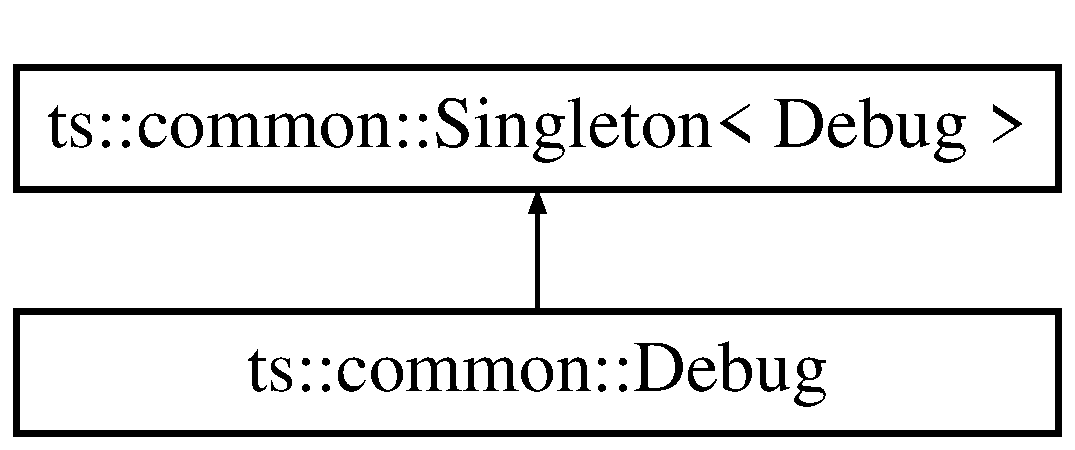
\includegraphics[height=2.000000cm]{classts_1_1common_1_1_debug}
\end{center}
\end{figure}
\subsection*{Public Types}
\begin{DoxyCompactItemize}
\item 
\mbox{\Hypertarget{classts_1_1common_1_1_debug_af0648abcd4bc4ae39293f0957caa2930}\label{classts_1_1common_1_1_debug_af0648abcd4bc4ae39293f0957caa2930}} 
enum {\bfseries Debug\+Type} \{ {\bfseries Error}, 
{\bfseries Warning}, 
{\bfseries Info}
 \}
\end{DoxyCompactItemize}
\subsection*{Public Member Functions}
\begin{DoxyCompactItemize}
\item 
\mbox{\Hypertarget{classts_1_1common_1_1_debug_a3440dbc6be1c1b605aff36c9b1d133e0}\label{classts_1_1common_1_1_debug_a3440dbc6be1c1b605aff36c9b1d133e0}} 
\hyperlink{classts_1_1common_1_1_debug}{Debug} \& {\bfseries set\+Type} (Debug\+Type type)
\item 
\mbox{\Hypertarget{classts_1_1common_1_1_debug_a82b2c8f2b6590845c22c83964d04a026}\label{classts_1_1common_1_1_debug_a82b2c8f2b6590845c22c83964d04a026}} 
{\footnotesize template$<$typename T\+Printable $>$ }\\\hyperlink{classts_1_1common_1_1_debug}{Debug} \& {\bfseries operator$<$$<$} (T\+Printable const \&obj)
\item 
\mbox{\Hypertarget{classts_1_1common_1_1_debug_ab30af1d3317a1a32622c8486f0df8161}\label{classts_1_1common_1_1_debug_ab30af1d3317a1a32622c8486f0df8161}} 
\hyperlink{classts_1_1common_1_1_debug}{Debug} \& {\bfseries operator$<$$<$} (std\+::ostream \&($\ast$os)(std\+::ostream \&))
\item 
\mbox{\Hypertarget{classts_1_1common_1_1_debug_a4113c8aa9bf0ebac5951a76dfb889ef5}\label{classts_1_1common_1_1_debug_a4113c8aa9bf0ebac5951a76dfb889ef5}} 
{\footnotesize template$<$typename T\+Printable $>$ }\\\hyperlink{classts_1_1common_1_1_debug}{Debug} \& {\bfseries log} (T\+Printable const \&obj)
\item 
\mbox{\Hypertarget{classts_1_1common_1_1_debug_aee4b0a4f8a2506f4af92c75bdf4746be}\label{classts_1_1common_1_1_debug_aee4b0a4f8a2506f4af92c75bdf4746be}} 
{\footnotesize template$<$typename T\+Printable $>$ }\\\hyperlink{classts_1_1common_1_1_debug}{Debug} \& {\bfseries log\+Warning} (T\+Printable const \&obj)
\item 
\mbox{\Hypertarget{classts_1_1common_1_1_debug_aefed563c3c179667062316a65f219f70}\label{classts_1_1common_1_1_debug_aefed563c3c179667062316a65f219f70}} 
{\footnotesize template$<$typename T\+Printable $>$ }\\\hyperlink{classts_1_1common_1_1_debug}{Debug} \& {\bfseries log\+Error} (T\+Printable const \&obj)
\item 
\mbox{\Hypertarget{classts_1_1common_1_1_debug_a1ce25fbe36ab47b629232d8131094b81}\label{classts_1_1common_1_1_debug_a1ce25fbe36ab47b629232d8131094b81}} 
{\footnotesize template$<$typename T\+Printable $>$ }\\\hyperlink{classts_1_1common_1_1_debug}{Debug} \& {\bfseries log\+Info} (T\+Printable const \&obj)
\item 
\mbox{\Hypertarget{classts_1_1common_1_1_debug_aac74d0240ee7ae82b54dd4d3657c7414}\label{classts_1_1common_1_1_debug_aac74d0240ee7ae82b54dd4d3657c7414}} 
{\bfseries Debug} (Debug\+Type type=Debug\+Type\+::\+Info)
\end{DoxyCompactItemize}
\subsection*{Static Public Member Functions}
\begin{DoxyCompactItemize}
\item 
\mbox{\Hypertarget{classts_1_1common_1_1_debug_a7d0f71910b5ab6aa5f00d743bdd3293d}\label{classts_1_1common_1_1_debug_a7d0f71910b5ab6aa5f00d743bdd3293d}} 
static void {\bfseries init} (Debug\+::\+Debug\+Type type, std\+::ostream \&os=std\+::cerr)
\end{DoxyCompactItemize}


The documentation for this class was generated from the following file\+:\begin{DoxyCompactItemize}
\item 
Util/Debug.\+hpp\end{DoxyCompactItemize}

\hypertarget{structts_1_1common_1_1_disconnect_req}{}\section{ts\+:\+:common\+:\+:Disconnect\+Req Struct Reference}
\label{structts_1_1common_1_1_disconnect_req}\index{ts\+::common\+::\+Disconnect\+Req@{ts\+::common\+::\+Disconnect\+Req}}
Inheritance diagram for ts\+:\+:common\+:\+:Disconnect\+Req\+:\begin{figure}[H]
\begin{center}
\leavevmode
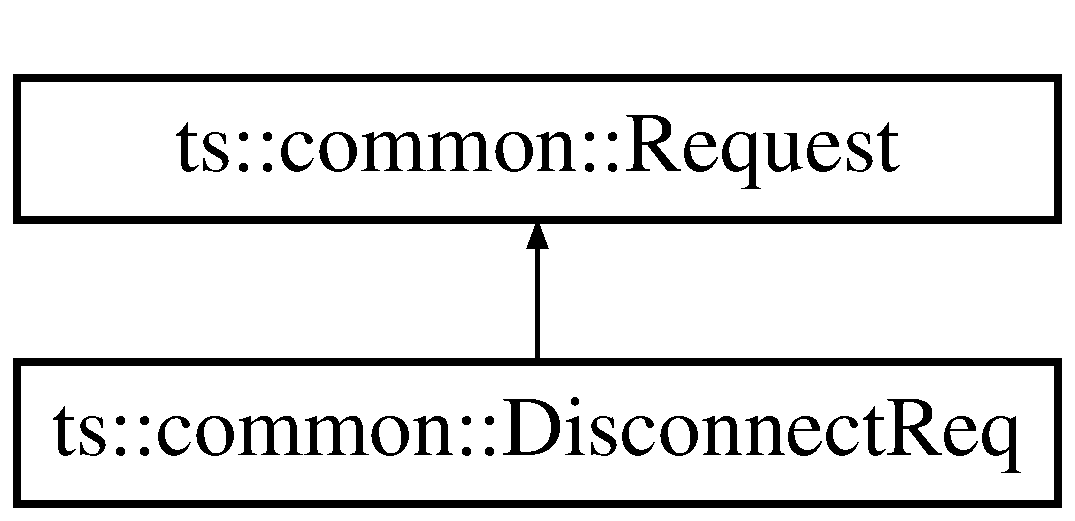
\includegraphics[height=2.000000cm]{structts_1_1common_1_1_disconnect_req}
\end{center}
\end{figure}
\subsection*{Public Member Functions}
\begin{DoxyCompactItemize}
\item 
\mbox{\Hypertarget{structts_1_1common_1_1_disconnect_req_aae1dfdccf2f82711fea48c93d0653af5}\label{structts_1_1common_1_1_disconnect_req_aae1dfdccf2f82711fea48c93d0653af5}} 
{\bfseries Disconnect\+Req} (std\+::string const \&from, std\+::string const \&to)
\item 
\mbox{\Hypertarget{structts_1_1common_1_1_disconnect_req_ad2c5dcc48f4e0ee16cb2846e1506e00f}\label{structts_1_1common_1_1_disconnect_req_ad2c5dcc48f4e0ee16cb2846e1506e00f}} 
int {\bfseries get\+Id} () const override
\item 
\mbox{\Hypertarget{structts_1_1common_1_1_disconnect_req_a3aa29c9e0f95bce40931dcece2a82ab6}\label{structts_1_1common_1_1_disconnect_req_a3aa29c9e0f95bce40931dcece2a82ab6}} 
void {\bfseries from\+Json} (std\+::string const \&json) override
\item 
\mbox{\Hypertarget{structts_1_1common_1_1_disconnect_req_af5496ad4f4a042827bc38fd57b71bc60}\label{structts_1_1common_1_1_disconnect_req_af5496ad4f4a042827bc38fd57b71bc60}} 
std\+::string {\bfseries to\+Json} () override
\end{DoxyCompactItemize}
\subsection*{Additional Inherited Members}


The documentation for this struct was generated from the following file\+:\begin{DoxyCompactItemize}
\item 
Request/Disconnect\+Req.\+hpp\end{DoxyCompactItemize}

\hypertarget{structts_1_1common_1_1_error_req}{}\section{ts\+:\+:common\+:\+:Error\+Req Struct Reference}
\label{structts_1_1common_1_1_error_req}\index{ts\+::common\+::\+Error\+Req@{ts\+::common\+::\+Error\+Req}}
Inheritance diagram for ts\+:\+:common\+:\+:Error\+Req\+:\begin{figure}[H]
\begin{center}
\leavevmode
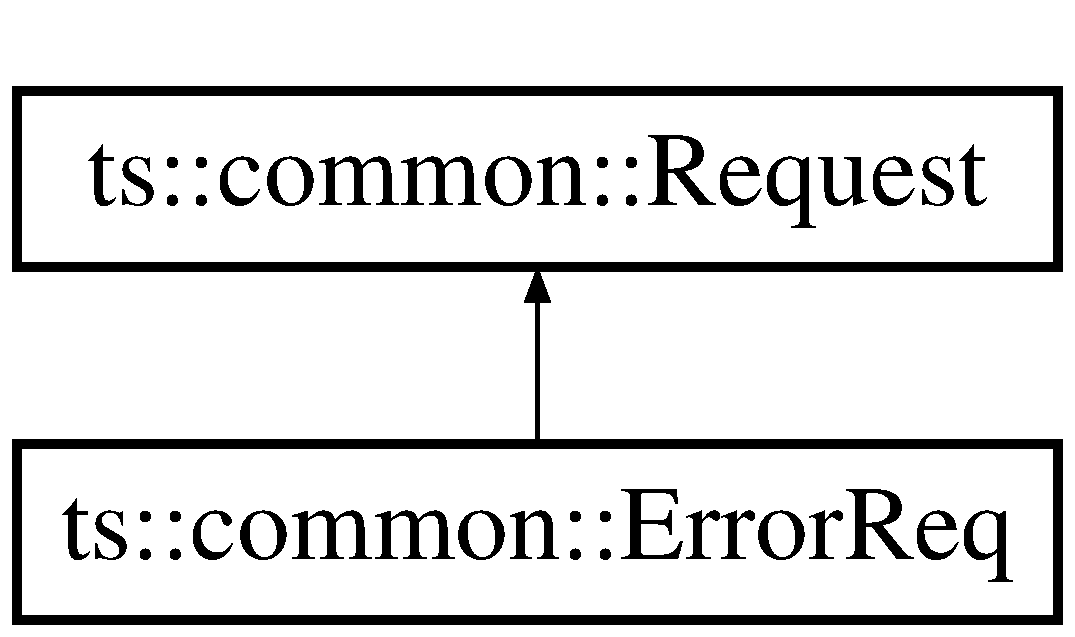
\includegraphics[height=2.000000cm]{structts_1_1common_1_1_error_req}
\end{center}
\end{figure}
\subsection*{Public Member Functions}
\begin{DoxyCompactItemize}
\item 
\mbox{\Hypertarget{structts_1_1common_1_1_error_req_a5bdeb0a76687e0e23b840064b873d343}\label{structts_1_1common_1_1_error_req_a5bdeb0a76687e0e23b840064b873d343}} 
{\bfseries Error\+Req} (std\+::string const \&from, std\+::string const \&to, Error\+Type error\+Type, std\+::string const \&message)
\item 
\mbox{\Hypertarget{structts_1_1common_1_1_error_req_a67b8214db379d0d61a1b421721936bda}\label{structts_1_1common_1_1_error_req_a67b8214db379d0d61a1b421721936bda}} 
int {\bfseries get\+Id} () const override
\item 
\mbox{\Hypertarget{structts_1_1common_1_1_error_req_af102b4aa668b10b75eeaf670e0614a44}\label{structts_1_1common_1_1_error_req_af102b4aa668b10b75eeaf670e0614a44}} 
void {\bfseries from\+Json} (std\+::string const \&json) override
\item 
\mbox{\Hypertarget{structts_1_1common_1_1_error_req_af42acd775e96ad61907815ab74ef3961}\label{structts_1_1common_1_1_error_req_af42acd775e96ad61907815ab74ef3961}} 
std\+::string {\bfseries to\+Json} () override
\end{DoxyCompactItemize}
\subsection*{Public Attributes}
\begin{DoxyCompactItemize}
\item 
\mbox{\Hypertarget{structts_1_1common_1_1_error_req_a0183447ba33cb20a07e73492070b017f}\label{structts_1_1common_1_1_error_req_a0183447ba33cb20a07e73492070b017f}} 
Error\+Type {\bfseries error\+Type}
\item 
\mbox{\Hypertarget{structts_1_1common_1_1_error_req_afe7707a51692975f1e221dd43504f799}\label{structts_1_1common_1_1_error_req_afe7707a51692975f1e221dd43504f799}} 
std\+::string {\bfseries message}
\end{DoxyCompactItemize}
\subsection*{Additional Inherited Members}


The documentation for this struct was generated from the following file\+:\begin{DoxyCompactItemize}
\item 
Request/Error\+Req.\+hpp\end{DoxyCompactItemize}

\hypertarget{classts_1_1_i_data_recorder}{}\section{ts\+:\+:I\+Data\+Recorder Class Reference}
\label{classts_1_1_i_data_recorder}\index{ts\+::\+I\+Data\+Recorder@{ts\+::\+I\+Data\+Recorder}}
Inheritance diagram for ts\+:\+:I\+Data\+Recorder\+:\begin{figure}[H]
\begin{center}
\leavevmode
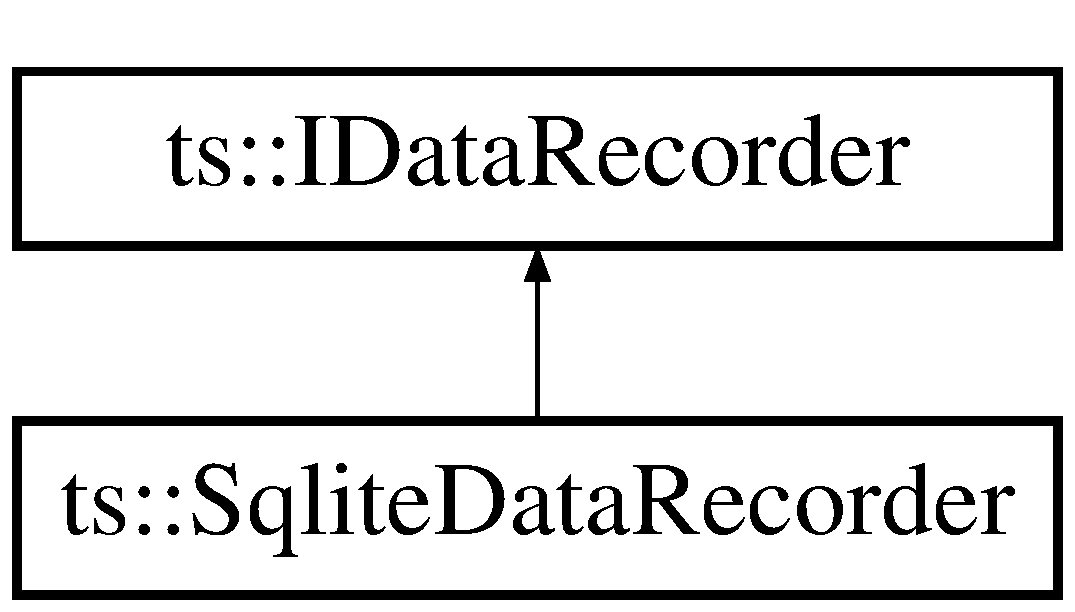
\includegraphics[height=2.000000cm]{classts_1_1_i_data_recorder}
\end{center}
\end{figure}
\subsection*{Public Member Functions}
\begin{DoxyCompactItemize}
\item 
\mbox{\Hypertarget{classts_1_1_i_data_recorder_a2d58e3018ea0b14d64eef86cb6bfd3fb}\label{classts_1_1_i_data_recorder_a2d58e3018ea0b14d64eef86cb6bfd3fb}} 
virtual void {\bfseries save} (\hyperlink{structts_1_1common_1_1_request}{common\+::\+Request} \&request)=0
\end{DoxyCompactItemize}


The documentation for this class was generated from the following file\+:\begin{DoxyCompactItemize}
\item 
Data\+Recorder/I\+Data\+Recorder.\+hpp\end{DoxyCompactItemize}

\hypertarget{classts_1_1common_1_1_json_parser}{}\section{ts\+:\+:common\+:\+:Json\+Parser Class Reference}
\label{classts_1_1common_1_1_json_parser}\index{ts\+::common\+::\+Json\+Parser@{ts\+::common\+::\+Json\+Parser}}
\subsection*{Public Member Functions}
\begin{DoxyCompactItemize}
\item 
void \hyperlink{classts_1_1common_1_1_json_parser_abba008df015d4baad7d03f0a03862ff9}{parse} (std\+::string const \&json)
\item 
{\footnotesize template$<$typename T\+Value $>$ }\\void \hyperlink{classts_1_1common_1_1_json_parser_a08607becc24052fb2c08cf583ac9b735}{get} (std\+::string const \&path, T\+Value \&value) const
\item 
{\footnotesize template$<$typename T\+Value , typename T\+Key  = T\+Value$>$ }\\void \hyperlink{classts_1_1common_1_1_json_parser_a3422774a1df58bbb3de563872f2d3841}{get} (std\+::string const \&path, std\+::vector$<$ std\+::pair$<$ T\+Key, T\+Value $>$$>$ \&values) const
\item 
{\footnotesize template$<$typename T\+Value $>$ }\\void \hyperlink{classts_1_1common_1_1_json_parser_aea9fd5f7744ff6a97075ebdb674f54df}{get} (std\+::string const \&path, std\+::vector$<$ T\+Value $>$ \&values)
\item 
\mbox{\Hypertarget{classts_1_1common_1_1_json_parser_a5397245ead2a54678856731f7a126f31}\label{classts_1_1common_1_1_json_parser_a5397245ead2a54678856731f7a126f31}} 
void \hyperlink{classts_1_1common_1_1_json_parser_a5397245ead2a54678856731f7a126f31}{clear} ()
\begin{DoxyCompactList}\small\item\em Clear data. \end{DoxyCompactList}\item 
{\footnotesize template$<$typename T\+Value $>$ }\\void \hyperlink{classts_1_1common_1_1_json_parser_acfb81f9e2bce7073b4f550b4cb99d21e}{put} (std\+::string const \&path, T\+Value const \&value)
\item 
\mbox{\Hypertarget{classts_1_1common_1_1_json_parser_acaa4bbc3d9de1c54c833282410f4152d}\label{classts_1_1common_1_1_json_parser_acaa4bbc3d9de1c54c833282410f4152d}} 
std\+::string \hyperlink{classts_1_1common_1_1_json_parser_acaa4bbc3d9de1c54c833282410f4152d}{write} ()
\begin{DoxyCompactList}\small\item\em Write the final json data. \end{DoxyCompactList}\end{DoxyCompactItemize}


\subsection{Member Function Documentation}
\mbox{\Hypertarget{classts_1_1common_1_1_json_parser_a08607becc24052fb2c08cf583ac9b735}\label{classts_1_1common_1_1_json_parser_a08607becc24052fb2c08cf583ac9b735}} 
\index{ts\+::common\+::\+Json\+Parser@{ts\+::common\+::\+Json\+Parser}!get@{get}}
\index{get@{get}!ts\+::common\+::\+Json\+Parser@{ts\+::common\+::\+Json\+Parser}}
\subsubsection{\texorpdfstring{get()}{get()}\hspace{0.1cm}{\footnotesize\ttfamily [1/3]}}
{\footnotesize\ttfamily template$<$typename T\+Value $>$ \\
void ts\+::common\+::\+Json\+Parser\+::get (\begin{DoxyParamCaption}\item[{std\+::string const \&}]{path,  }\item[{T\+Value \&}]{value }\end{DoxyParamCaption}) const\hspace{0.3cm}{\ttfamily [inline]}}

Get a value 
\begin{DoxyTemplParams}{Template Parameters}
{\em T\+Value} & \\
\hline
\end{DoxyTemplParams}

\begin{DoxyParams}{Parameters}
{\em path} & \\
\hline
{\em value} & \\
\hline
\end{DoxyParams}
\mbox{\Hypertarget{classts_1_1common_1_1_json_parser_a3422774a1df58bbb3de563872f2d3841}\label{classts_1_1common_1_1_json_parser_a3422774a1df58bbb3de563872f2d3841}} 
\index{ts\+::common\+::\+Json\+Parser@{ts\+::common\+::\+Json\+Parser}!get@{get}}
\index{get@{get}!ts\+::common\+::\+Json\+Parser@{ts\+::common\+::\+Json\+Parser}}
\subsubsection{\texorpdfstring{get()}{get()}\hspace{0.1cm}{\footnotesize\ttfamily [2/3]}}
{\footnotesize\ttfamily template$<$typename T\+Value , typename T\+Key  = T\+Value$>$ \\
void ts\+::common\+::\+Json\+Parser\+::get (\begin{DoxyParamCaption}\item[{std\+::string const \&}]{path,  }\item[{std\+::vector$<$ std\+::pair$<$ T\+Key, T\+Value $>$$>$ \&}]{values }\end{DoxyParamCaption}) const\hspace{0.3cm}{\ttfamily [inline]}}

Get a value 
\begin{DoxyTemplParams}{Template Parameters}
{\em T\+Value} & \\
\hline
{\em T\+Key} & \\
\hline
\end{DoxyTemplParams}

\begin{DoxyParams}{Parameters}
{\em path} & \\
\hline
{\em values} & \\
\hline
\end{DoxyParams}
\mbox{\Hypertarget{classts_1_1common_1_1_json_parser_aea9fd5f7744ff6a97075ebdb674f54df}\label{classts_1_1common_1_1_json_parser_aea9fd5f7744ff6a97075ebdb674f54df}} 
\index{ts\+::common\+::\+Json\+Parser@{ts\+::common\+::\+Json\+Parser}!get@{get}}
\index{get@{get}!ts\+::common\+::\+Json\+Parser@{ts\+::common\+::\+Json\+Parser}}
\subsubsection{\texorpdfstring{get()}{get()}\hspace{0.1cm}{\footnotesize\ttfamily [3/3]}}
{\footnotesize\ttfamily template$<$typename T\+Value $>$ \\
void ts\+::common\+::\+Json\+Parser\+::get (\begin{DoxyParamCaption}\item[{std\+::string const \&}]{path,  }\item[{std\+::vector$<$ T\+Value $>$ \&}]{values }\end{DoxyParamCaption})\hspace{0.3cm}{\ttfamily [inline]}}

Get a value 
\begin{DoxyTemplParams}{Template Parameters}
{\em T\+Value} & \\
\hline
\end{DoxyTemplParams}

\begin{DoxyParams}{Parameters}
{\em path} & \\
\hline
{\em values} & \\
\hline
\end{DoxyParams}
\mbox{\Hypertarget{classts_1_1common_1_1_json_parser_abba008df015d4baad7d03f0a03862ff9}\label{classts_1_1common_1_1_json_parser_abba008df015d4baad7d03f0a03862ff9}} 
\index{ts\+::common\+::\+Json\+Parser@{ts\+::common\+::\+Json\+Parser}!parse@{parse}}
\index{parse@{parse}!ts\+::common\+::\+Json\+Parser@{ts\+::common\+::\+Json\+Parser}}
\subsubsection{\texorpdfstring{parse()}{parse()}}
{\footnotesize\ttfamily void ts\+::common\+::\+Json\+Parser\+::parse (\begin{DoxyParamCaption}\item[{std\+::string const \&}]{json }\end{DoxyParamCaption})}

Parse the json 
\begin{DoxyParams}{Parameters}
{\em json} & \\
\hline
\end{DoxyParams}
\mbox{\Hypertarget{classts_1_1common_1_1_json_parser_acfb81f9e2bce7073b4f550b4cb99d21e}\label{classts_1_1common_1_1_json_parser_acfb81f9e2bce7073b4f550b4cb99d21e}} 
\index{ts\+::common\+::\+Json\+Parser@{ts\+::common\+::\+Json\+Parser}!put@{put}}
\index{put@{put}!ts\+::common\+::\+Json\+Parser@{ts\+::common\+::\+Json\+Parser}}
\subsubsection{\texorpdfstring{put()}{put()}}
{\footnotesize\ttfamily template$<$typename T\+Value $>$ \\
void ts\+::common\+::\+Json\+Parser\+::put (\begin{DoxyParamCaption}\item[{std\+::string const \&}]{path,  }\item[{T\+Value const \&}]{value }\end{DoxyParamCaption})\hspace{0.3cm}{\ttfamily [inline]}}

Add new json entry 
\begin{DoxyTemplParams}{Template Parameters}
{\em T\+Value} & \\
\hline
\end{DoxyTemplParams}

\begin{DoxyParams}{Parameters}
{\em path} & \\
\hline
{\em value} & \\
\hline
\end{DoxyParams}


The documentation for this class was generated from the following file\+:\begin{DoxyCompactItemize}
\item 
Json/Json\+Parser.\+hpp\end{DoxyCompactItemize}

\hypertarget{structts_1_1common_1_1_key_info_req}{}\section{ts\+:\+:common\+:\+:Key\+Info\+Req Struct Reference}
\label{structts_1_1common_1_1_key_info_req}\index{ts\+::common\+::\+Key\+Info\+Req@{ts\+::common\+::\+Key\+Info\+Req}}
Inheritance diagram for ts\+:\+:common\+:\+:Key\+Info\+Req\+:\begin{figure}[H]
\begin{center}
\leavevmode
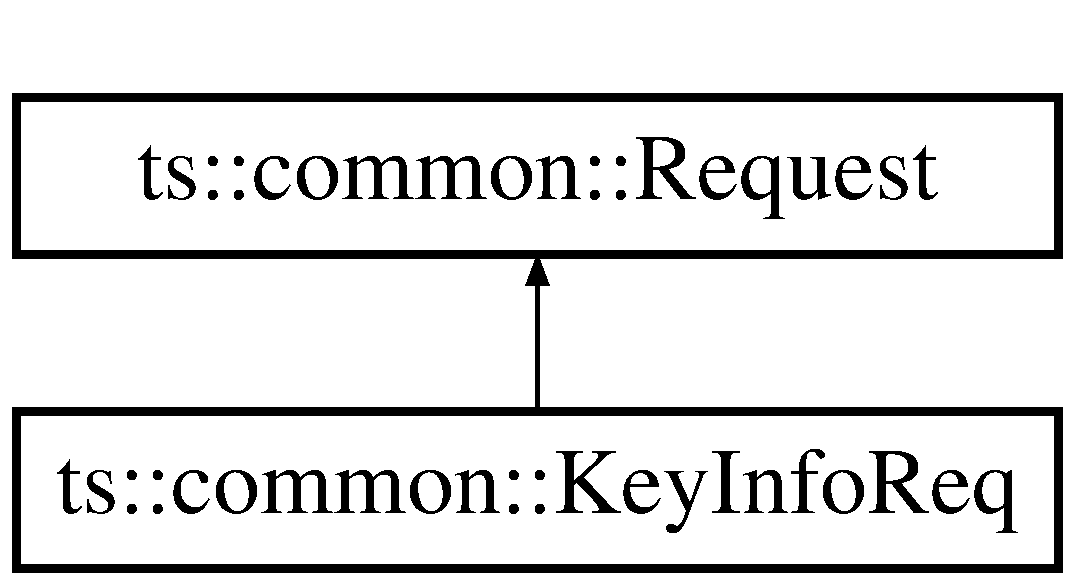
\includegraphics[height=2.000000cm]{structts_1_1common_1_1_key_info_req}
\end{center}
\end{figure}
\subsection*{Public Member Functions}
\begin{DoxyCompactItemize}
\item 
\mbox{\Hypertarget{structts_1_1common_1_1_key_info_req_a53639a1233c987a687a953f28b65a3f4}\label{structts_1_1common_1_1_key_info_req_a53639a1233c987a687a953f28b65a3f4}} 
{\bfseries Key\+Info\+Req} (std\+::string const \&from, std\+::string const \&to, std\+::string const \&keys, std\+::string const \&process\+Info)
\item 
\mbox{\Hypertarget{structts_1_1common_1_1_key_info_req_a01d7af709eca139df7e0fc42540aa31c}\label{structts_1_1common_1_1_key_info_req_a01d7af709eca139df7e0fc42540aa31c}} 
int {\bfseries get\+Id} () const override
\item 
\mbox{\Hypertarget{structts_1_1common_1_1_key_info_req_a69aeb081d361836cf8d4e6fabb7d6812}\label{structts_1_1common_1_1_key_info_req_a69aeb081d361836cf8d4e6fabb7d6812}} 
void {\bfseries from\+Json} (std\+::string const \&json) override
\item 
\mbox{\Hypertarget{structts_1_1common_1_1_key_info_req_af6dde21ab32464de8dd56ab41895046e}\label{structts_1_1common_1_1_key_info_req_af6dde21ab32464de8dd56ab41895046e}} 
std\+::string {\bfseries to\+Json} () override
\end{DoxyCompactItemize}
\subsection*{Public Attributes}
\begin{DoxyCompactItemize}
\item 
\mbox{\Hypertarget{structts_1_1common_1_1_key_info_req_aa1b2351c9e16670d8482e84095ff9f63}\label{structts_1_1common_1_1_key_info_req_aa1b2351c9e16670d8482e84095ff9f63}} 
std\+::string {\bfseries keys}
\item 
\mbox{\Hypertarget{structts_1_1common_1_1_key_info_req_adbeedc415e2c74202a14ace7e836f605}\label{structts_1_1common_1_1_key_info_req_adbeedc415e2c74202a14ace7e836f605}} 
std\+::string {\bfseries process\+Info}
\end{DoxyCompactItemize}
\subsection*{Additional Inherited Members}


The documentation for this struct was generated from the following file\+:\begin{DoxyCompactItemize}
\item 
Request/Key\+Info\+Req.\+hpp\end{DoxyCompactItemize}

\hypertarget{structts_1_1common_1_1_notice_receipt_req}{}\section{ts\+:\+:common\+:\+:Notice\+Receipt\+Req Struct Reference}
\label{structts_1_1common_1_1_notice_receipt_req}\index{ts\+::common\+::\+Notice\+Receipt\+Req@{ts\+::common\+::\+Notice\+Receipt\+Req}}
Inheritance diagram for ts\+:\+:common\+:\+:Notice\+Receipt\+Req\+:\begin{figure}[H]
\begin{center}
\leavevmode
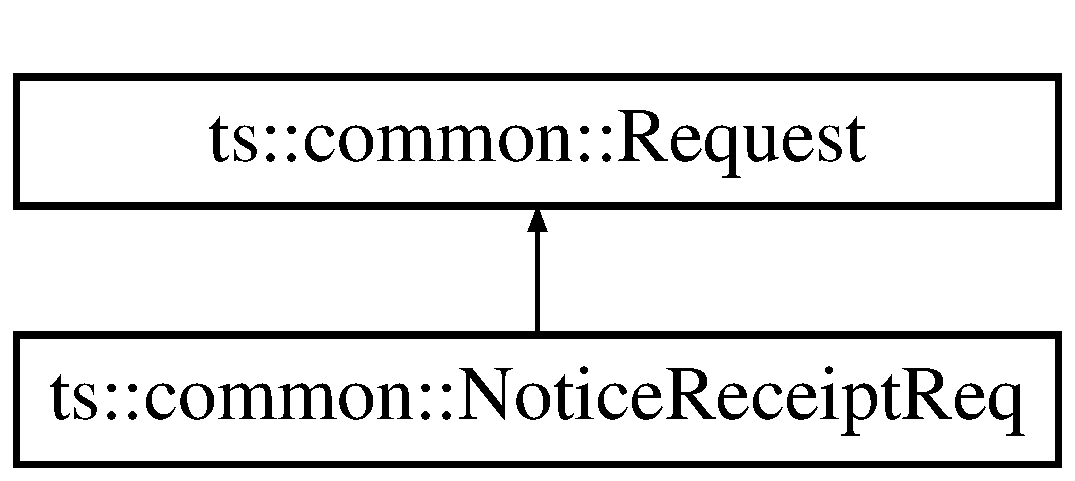
\includegraphics[height=2.000000cm]{structts_1_1common_1_1_notice_receipt_req}
\end{center}
\end{figure}
\subsection*{Public Member Functions}
\begin{DoxyCompactItemize}
\item 
\mbox{\Hypertarget{structts_1_1common_1_1_notice_receipt_req_ae3a269817ffc1f31bc2f86dba3c39c87}\label{structts_1_1common_1_1_notice_receipt_req_ae3a269817ffc1f31bc2f86dba3c39c87}} 
{\bfseries Notice\+Receipt\+Req} (std\+::string const \&from, std\+::string const \&to, unsigned int req\+Timestamp, int req\+Id)
\item 
\mbox{\Hypertarget{structts_1_1common_1_1_notice_receipt_req_a4b2e55b26d5c4ed005d787369afc8622}\label{structts_1_1common_1_1_notice_receipt_req_a4b2e55b26d5c4ed005d787369afc8622}} 
int {\bfseries get\+Id} () const override
\item 
\mbox{\Hypertarget{structts_1_1common_1_1_notice_receipt_req_a5b4cde4c42fc619e4a540754d6517998}\label{structts_1_1common_1_1_notice_receipt_req_a5b4cde4c42fc619e4a540754d6517998}} 
void {\bfseries from\+Json} (std\+::string const \&json) override
\item 
\mbox{\Hypertarget{structts_1_1common_1_1_notice_receipt_req_ab463957c39288f188e569178dce17e8a}\label{structts_1_1common_1_1_notice_receipt_req_ab463957c39288f188e569178dce17e8a}} 
std\+::string {\bfseries to\+Json} () override
\end{DoxyCompactItemize}
\subsection*{Public Attributes}
\begin{DoxyCompactItemize}
\item 
\mbox{\Hypertarget{structts_1_1common_1_1_notice_receipt_req_acd41c25edaeaac9666e94002dfe9fbd9}\label{structts_1_1common_1_1_notice_receipt_req_acd41c25edaeaac9666e94002dfe9fbd9}} 
unsigned int {\bfseries req\+Timestamp}
\item 
\mbox{\Hypertarget{structts_1_1common_1_1_notice_receipt_req_a0c8466461bb115c2f0c336be4956e0e3}\label{structts_1_1common_1_1_notice_receipt_req_a0c8466461bb115c2f0c336be4956e0e3}} 
int {\bfseries req\+Id}
\end{DoxyCompactItemize}
\subsection*{Additional Inherited Members}


The documentation for this struct was generated from the following file\+:\begin{DoxyCompactItemize}
\item 
Request/Notice\+Receipt\+Req.\+hpp\end{DoxyCompactItemize}

\hypertarget{structts_1_1_option}{}\section{ts\+:\+:Option Struct Reference}
\label{structts_1_1_option}\index{ts\+::\+Option@{ts\+::\+Option}}
\subsection*{Public Member Functions}
\begin{DoxyCompactItemize}
\item 
\mbox{\Hypertarget{structts_1_1_option_aceef3c5ffc2f332aa3e2350f61abfe75}\label{structts_1_1_option_aceef3c5ffc2f332aa3e2350f61abfe75}} 
{\bfseries Option} (std\+::string const \&description=\char`\"{}\char`\"{}, std\+::string const \&name=\char`\"{}\char`\"{}, std\+::string short\+Name=\char`\"{}\char`\"{})
\item 
\mbox{\Hypertarget{structts_1_1_option_a6bbab372f320c3e290c8d7665f6b771c}\label{structts_1_1_option_a6bbab372f320c3e290c8d7665f6b771c}} 
bool {\bfseries is\+Required} () const
\item 
\mbox{\Hypertarget{structts_1_1_option_ab72f836e79c97a0701a7297b64ba4cbe}\label{structts_1_1_option_ab72f836e79c97a0701a7297b64ba4cbe}} 
bool {\bfseries has\+Value} () const
\item 
\mbox{\Hypertarget{structts_1_1_option_a71e8f36453f42f0bc0ce714b381af87c}\label{structts_1_1_option_a71e8f36453f42f0bc0ce714b381af87c}} 
void {\bfseries set\+Is\+Required} (bool state)
\item 
\mbox{\Hypertarget{structts_1_1_option_ac860f059ba576ad8d8a206c7aef2c026}\label{structts_1_1_option_ac860f059ba576ad8d8a206c7aef2c026}} 
void {\bfseries set\+Has\+Value} (bool state)
\end{DoxyCompactItemize}
\subsection*{Public Attributes}
\begin{DoxyCompactItemize}
\item 
\mbox{\Hypertarget{structts_1_1_option_a2fb94cede2b4c8eb012013bc01d6c1c9}\label{structts_1_1_option_a2fb94cede2b4c8eb012013bc01d6c1c9}} 
std\+::string {\bfseries name}
\item 
\mbox{\Hypertarget{structts_1_1_option_a6337eaf84d124c11c028b5a1d8db4d75}\label{structts_1_1_option_a6337eaf84d124c11c028b5a1d8db4d75}} 
std\+::string {\bfseries short\+Name}
\item 
\mbox{\Hypertarget{structts_1_1_option_a3e4741cd5d3555da48762f6534463e14}\label{structts_1_1_option_a3e4741cd5d3555da48762f6534463e14}} 
std\+::string {\bfseries description}
\end{DoxyCompactItemize}
\subsection*{Protected Attributes}
\begin{DoxyCompactItemize}
\item 
\mbox{\Hypertarget{structts_1_1_option_a37a2229e1048b8f8f2acc9f72990f00f}\label{structts_1_1_option_a37a2229e1048b8f8f2acc9f72990f00f}} 
bool {\bfseries required}
\item 
\mbox{\Hypertarget{structts_1_1_option_affdb2491c28f14eaf43c50b2f674a676}\label{structts_1_1_option_affdb2491c28f14eaf43c50b2f674a676}} 
bool {\bfseries with\+Value}
\end{DoxyCompactItemize}


The documentation for this struct was generated from the following file\+:\begin{DoxyCompactItemize}
\item 
Program\+Option/Option.\+hpp\end{DoxyCompactItemize}

\hypertarget{structts_1_1common_1_1_packet}{}\section{ts\+:\+:common\+:\+:Packet Struct Reference}
\label{structts_1_1common_1_1_packet}\index{ts\+::common\+::\+Packet@{ts\+::common\+::\+Packet}}
\subsection*{Public Attributes}
\begin{DoxyCompactItemize}
\item 
\mbox{\Hypertarget{structts_1_1common_1_1_packet_a22cf5cbe00488c2f324bc580b43b332b}\label{structts_1_1common_1_1_packet_a22cf5cbe00488c2f324bc580b43b332b}} 
\hyperlink{structts_1_1common_1_1_packet_header}{Packet\+Header} {\bfseries header} \{\}
\item 
\mbox{\Hypertarget{structts_1_1common_1_1_packet_ae1df6eb6a4d7307e68369a144a0c6a51}\label{structts_1_1common_1_1_packet_ae1df6eb6a4d7307e68369a144a0c6a51}} 
\hyperlink{structts_1_1common_1_1_packet_body}{Packet\+Body} {\bfseries body} \{\}
\end{DoxyCompactItemize}


The documentation for this struct was generated from the following file\+:\begin{DoxyCompactItemize}
\item 
Socket/Packet.\+hpp\end{DoxyCompactItemize}

\hypertarget{structts_1_1common_1_1_packet_body}{}\section{ts\+:\+:common\+:\+:Packet\+Body Struct Reference}
\label{structts_1_1common_1_1_packet_body}\index{ts\+::common\+::\+Packet\+Body@{ts\+::common\+::\+Packet\+Body}}
\subsection*{Public Member Functions}
\begin{DoxyCompactItemize}
\item 
\mbox{\Hypertarget{structts_1_1common_1_1_packet_body_a2a7de4788181d825b0187aabe71354ec}\label{structts_1_1common_1_1_packet_body_a2a7de4788181d825b0187aabe71354ec}} 
void \hyperlink{structts_1_1common_1_1_packet_body_a2a7de4788181d825b0187aabe71354ec}{reset} ()
\begin{DoxyCompactList}\small\item\em Reset data in body. \end{DoxyCompactList}\end{DoxyCompactItemize}
\subsection*{Public Attributes}
\begin{DoxyCompactItemize}
\item 
\mbox{\Hypertarget{structts_1_1common_1_1_packet_body_ac209e31fb1a4d1024061a4949d923ff0}\label{structts_1_1common_1_1_packet_body_ac209e31fb1a4d1024061a4949d923ff0}} 
char $\ast$ {\bfseries data}
\end{DoxyCompactItemize}


The documentation for this struct was generated from the following file\+:\begin{DoxyCompactItemize}
\item 
Packet/Packet.\+hpp\end{DoxyCompactItemize}

\hypertarget{structts_1_1common_1_1_packet_header}{}\section{ts\+:\+:common\+:\+:Packet\+Header Struct Reference}
\label{structts_1_1common_1_1_packet_header}\index{ts\+::common\+::\+Packet\+Header@{ts\+::common\+::\+Packet\+Header}}
\subsection*{Public Member Functions}
\begin{DoxyCompactItemize}
\item 
\mbox{\Hypertarget{structts_1_1common_1_1_packet_header_adf4e5e691171eeac8d38f8d0ddf3e138}\label{structts_1_1common_1_1_packet_header_adf4e5e691171eeac8d38f8d0ddf3e138}} 
void \hyperlink{structts_1_1common_1_1_packet_header_adf4e5e691171eeac8d38f8d0ddf3e138}{reset} ()
\begin{DoxyCompactList}\small\item\em Reset data in header. \end{DoxyCompactList}\end{DoxyCompactItemize}
\subsection*{Public Attributes}
\begin{DoxyCompactItemize}
\item 
\mbox{\Hypertarget{structts_1_1common_1_1_packet_header_a95214ffcb1c52edd7a6282c2e6a40025}\label{structts_1_1common_1_1_packet_header_a95214ffcb1c52edd7a6282c2e6a40025}} 
int {\bfseries id}
\item 
\mbox{\Hypertarget{structts_1_1common_1_1_packet_header_a5dc7af4be3fbff0ca3756202450fe882}\label{structts_1_1common_1_1_packet_header_a5dc7af4be3fbff0ca3756202450fe882}} 
int {\bfseries size}
\end{DoxyCompactItemize}


The documentation for this struct was generated from the following file\+:\begin{DoxyCompactItemize}
\item 
Packet/Packet.\+hpp\end{DoxyCompactItemize}

\hypertarget{classts_1_1common_1_1_packet_manager}{}\section{ts\+:\+:common\+:\+:Packet\+Manager Class Reference}
\label{classts_1_1common_1_1_packet_manager}\index{ts\+::common\+::\+Packet\+Manager@{ts\+::common\+::\+Packet\+Manager}}
\subsection*{Public Member Functions}
\begin{DoxyCompactItemize}
\item 
\mbox{\Hypertarget{classts_1_1common_1_1_packet_manager_a3b73116e602124697590afecb82ef9fd}\label{classts_1_1common_1_1_packet_manager_a3b73116e602124697590afecb82ef9fd}} 
{\bfseries Packet\+Manager} (\hyperlink{classts_1_1common_1_1tcp_1_1_client_socket}{common\+::tcp\+::\+Client\+Socket} \&client\+Socket)
\item 
\mbox{\Hypertarget{classts_1_1common_1_1_packet_manager_a6165799da03af1c119d921ac96a24562}\label{classts_1_1common_1_1_packet_manager_a6165799da03af1c119d921ac96a24562}} 
void {\bfseries async\+Read} (On\+Read\+Complete\+Packet on\+Read\+Complete\+Packet, On\+Read\+Packet\+Error on\+Read\+Packet\+Error)
\item 
\mbox{\Hypertarget{classts_1_1common_1_1_packet_manager_ae308b816f8cf10367f0f63fa5c1fadf4}\label{classts_1_1common_1_1_packet_manager_ae308b816f8cf10367f0f63fa5c1fadf4}} 
void {\bfseries async\+Write} (std\+::shared\+\_\+ptr$<$ \hyperlink{structts_1_1common_1_1_packet}{Packet} $>$ const \&packet, On\+Write\+Complete\+Packet on\+Write\+Complete\+Packet, On\+Write\+Packet\+Error on\+Write\+Packet\+Error)
\item 
\mbox{\Hypertarget{classts_1_1common_1_1_packet_manager_aae446c8e99adc8ead7d4b0cd40545cd0}\label{classts_1_1common_1_1_packet_manager_aae446c8e99adc8ead7d4b0cd40545cd0}} 
void {\bfseries send} (int packet\+Header\+Id, std\+::string const \&data, On\+Write\+Complete\+Packet on\+Write\+Complete\+Packet, On\+Write\+Packet\+Error on\+Write\+Packet\+Error)
\end{DoxyCompactItemize}


The documentation for this class was generated from the following file\+:\begin{DoxyCompactItemize}
\item 
Socket/Packet\+Manager.\+hpp\end{DoxyCompactItemize}

\hypertarget{structts_1_1common_1_1_ping_req}{}\section{ts\+:\+:common\+:\+:Ping\+Req Struct Reference}
\label{structts_1_1common_1_1_ping_req}\index{ts\+::common\+::\+Ping\+Req@{ts\+::common\+::\+Ping\+Req}}
Inheritance diagram for ts\+:\+:common\+:\+:Ping\+Req\+:\begin{figure}[H]
\begin{center}
\leavevmode
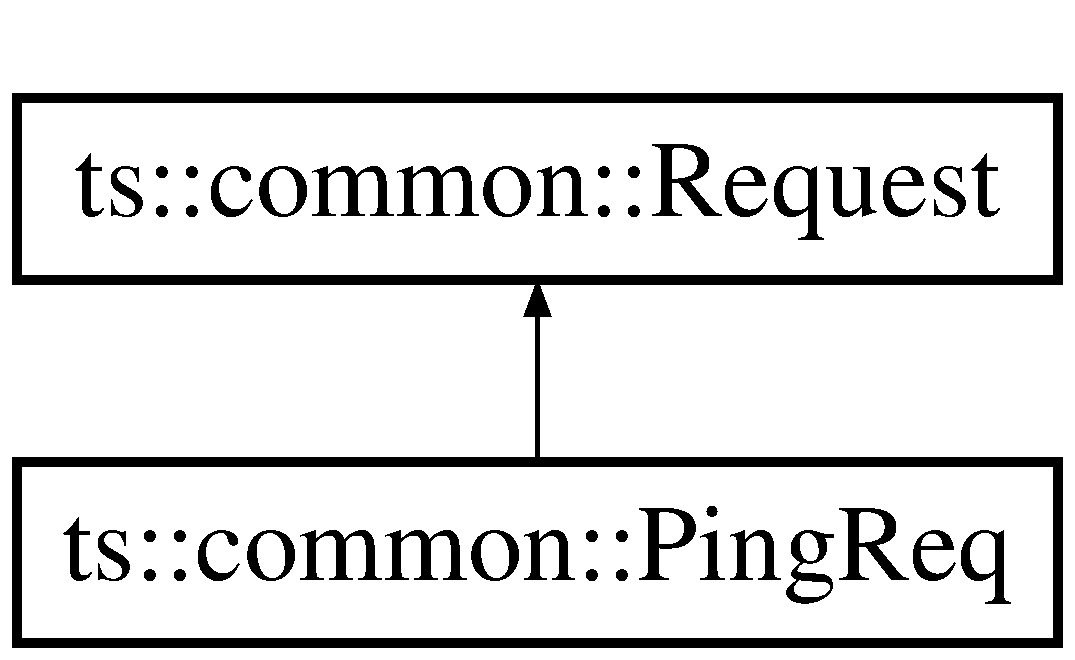
\includegraphics[height=2.000000cm]{structts_1_1common_1_1_ping_req}
\end{center}
\end{figure}
\subsection*{Public Member Functions}
\begin{DoxyCompactItemize}
\item 
\mbox{\Hypertarget{structts_1_1common_1_1_ping_req_a9086ad567570fee92409bb791666ce38}\label{structts_1_1common_1_1_ping_req_a9086ad567570fee92409bb791666ce38}} 
{\bfseries Ping\+Req} (std\+::string const \&from, std\+::string const \&to)
\item 
\mbox{\Hypertarget{structts_1_1common_1_1_ping_req_aade4de990031733abcb7257744eeeae4}\label{structts_1_1common_1_1_ping_req_aade4de990031733abcb7257744eeeae4}} 
int {\bfseries get\+Id} () const override
\item 
\mbox{\Hypertarget{structts_1_1common_1_1_ping_req_a42de7cb0b189a256a844d26fd5c5e498}\label{structts_1_1common_1_1_ping_req_a42de7cb0b189a256a844d26fd5c5e498}} 
void {\bfseries from\+Json} (std\+::string const \&json) override
\item 
\mbox{\Hypertarget{structts_1_1common_1_1_ping_req_ab839ec43a055496f39fa209654ae4a6a}\label{structts_1_1common_1_1_ping_req_ab839ec43a055496f39fa209654ae4a6a}} 
std\+::string {\bfseries to\+Json} () override
\end{DoxyCompactItemize}
\subsection*{Additional Inherited Members}


The documentation for this struct was generated from the following file\+:\begin{DoxyCompactItemize}
\item 
Request/Ping\+Req.\+hpp\end{DoxyCompactItemize}

\hypertarget{structts_1_1common_1_1_ping_resp}{}\section{ts\+:\+:common\+:\+:Ping\+Resp Struct Reference}
\label{structts_1_1common_1_1_ping_resp}\index{ts\+::common\+::\+Ping\+Resp@{ts\+::common\+::\+Ping\+Resp}}
Inheritance diagram for ts\+:\+:common\+:\+:Ping\+Resp\+:\begin{figure}[H]
\begin{center}
\leavevmode
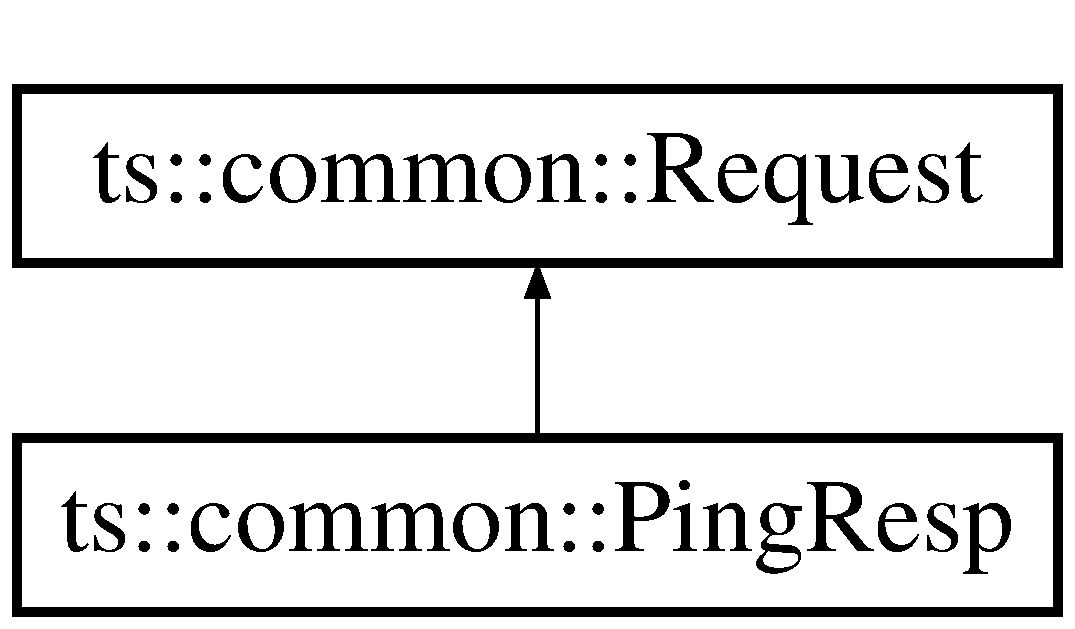
\includegraphics[height=2.000000cm]{structts_1_1common_1_1_ping_resp}
\end{center}
\end{figure}
\subsection*{Public Member Functions}
\begin{DoxyCompactItemize}
\item 
\mbox{\Hypertarget{structts_1_1common_1_1_ping_resp_a3e05fef64cc758593e380d63c9db3a39}\label{structts_1_1common_1_1_ping_resp_a3e05fef64cc758593e380d63c9db3a39}} 
{\bfseries Ping\+Resp} (std\+::string const \&from, std\+::string const \&to)
\item 
\mbox{\Hypertarget{structts_1_1common_1_1_ping_resp_af57c3c4e352c3b86e2c380506eb257be}\label{structts_1_1common_1_1_ping_resp_af57c3c4e352c3b86e2c380506eb257be}} 
int {\bfseries get\+Id} () const override
\item 
\mbox{\Hypertarget{structts_1_1common_1_1_ping_resp_a890c9c10fc302185d059af03bebbb79f}\label{structts_1_1common_1_1_ping_resp_a890c9c10fc302185d059af03bebbb79f}} 
void {\bfseries from\+Json} (std\+::string const \&json) override
\item 
\mbox{\Hypertarget{structts_1_1common_1_1_ping_resp_ab0d431ae3c8cbdf197c34579b901c7ca}\label{structts_1_1common_1_1_ping_resp_ab0d431ae3c8cbdf197c34579b901c7ca}} 
std\+::string {\bfseries to\+Json} () override
\end{DoxyCompactItemize}
\subsection*{Additional Inherited Members}


The documentation for this struct was generated from the following file\+:\begin{DoxyCompactItemize}
\item 
Request/Ping\+Resp.\+hpp\end{DoxyCompactItemize}

\hypertarget{classts_1_1_program_option}{}\section{ts\+:\+:Program\+Option Class Reference}
\label{classts_1_1_program_option}\index{ts\+::\+Program\+Option@{ts\+::\+Program\+Option}}
\subsection*{Public Member Functions}
\begin{DoxyCompactItemize}
\item 
\mbox{\Hypertarget{classts_1_1_program_option_a5aa7d69a91efcef19deb1a281950bac2}\label{classts_1_1_program_option_a5aa7d69a91efcef19deb1a281950bac2}} 
{\bfseries Program\+Option} (int ac, char const $\ast$$\ast$av)
\item 
\mbox{\Hypertarget{classts_1_1_program_option_a337d103d0a77405e32e947099c4c3c7c}\label{classts_1_1_program_option_a337d103d0a77405e32e947099c4c3c7c}} 
{\footnotesize template$<$typename T\+Value $>$ }\\void {\bfseries add\+Option} (\hyperlink{structts_1_1_option}{Option} \&option)
\item 
\mbox{\Hypertarget{classts_1_1_program_option_a23ae65a443f6aeed2b748b14802d75e2}\label{classts_1_1_program_option_a23ae65a443f6aeed2b748b14802d75e2}} 
{\footnotesize template$<$typename T\+Value $>$ }\\void {\bfseries add\+Option} (\hyperlink{structts_1_1_option}{Option} \&option, T\+Value const \&default\+Value)
\item 
\mbox{\Hypertarget{classts_1_1_program_option_ac79eaeb10a191f5fb83d35f4d35beae9}\label{classts_1_1_program_option_ac79eaeb10a191f5fb83d35f4d35beae9}} 
void {\bfseries add\+Option} (\hyperlink{structts_1_1_option}{Option} const \&option)
\item 
\mbox{\Hypertarget{classts_1_1_program_option_a37061a42e9fedbc863cf50a60737761c}\label{classts_1_1_program_option_a37061a42e9fedbc863cf50a60737761c}} 
void {\bfseries run} ()
\item 
\mbox{\Hypertarget{classts_1_1_program_option_a8b1d004f4a02f9688988a3aeb6058a77}\label{classts_1_1_program_option_a8b1d004f4a02f9688988a3aeb6058a77}} 
void {\bfseries print\+Option\+Description} (std\+::ostream \&out=std\+::cout) const
\item 
\mbox{\Hypertarget{classts_1_1_program_option_a8fc28b81bf1ced5970c594d93de3a69c}\label{classts_1_1_program_option_a8fc28b81bf1ced5970c594d93de3a69c}} 
void {\bfseries print\+Program\+Arguments} (std\+::ostream \&out=std\+::cout) const
\item 
\mbox{\Hypertarget{classts_1_1_program_option_ad08d06421491f66e936f597bd4298c43}\label{classts_1_1_program_option_ad08d06421491f66e936f597bd4298c43}} 
void {\bfseries print\+Usage} (std\+::ostream \&out=std\+::cout) const
\item 
\mbox{\Hypertarget{classts_1_1_program_option_a1fb7f75c8ac5456b83658f05530c3fb1}\label{classts_1_1_program_option_a1fb7f75c8ac5456b83658f05530c3fb1}} 
bool {\bfseries has} (std\+::string const \&name, std\+::string const \&short\+Name=\char`\"{}\char`\"{}) const
\item 
\mbox{\Hypertarget{classts_1_1_program_option_a942871d06299c44198a284761c8aa6dc}\label{classts_1_1_program_option_a942871d06299c44198a284761c8aa6dc}} 
{\footnotesize template$<$typename T\+Value $>$ }\\T\+Value {\bfseries get} (std\+::string const \&name, std\+::string const \&short\+Name=\char`\"{}\char`\"{})
\end{DoxyCompactItemize}


The documentation for this class was generated from the following file\+:\begin{DoxyCompactItemize}
\item 
Program\+Option/Program\+Option.\+hpp\end{DoxyCompactItemize}

\hypertarget{classts_1_1_program_option_exception}{}\section{ts\+:\+:Program\+Option\+Exception Class Reference}
\label{classts_1_1_program_option_exception}\index{ts\+::\+Program\+Option\+Exception@{ts\+::\+Program\+Option\+Exception}}
Inheritance diagram for ts\+:\+:Program\+Option\+Exception\+:\begin{figure}[H]
\begin{center}
\leavevmode
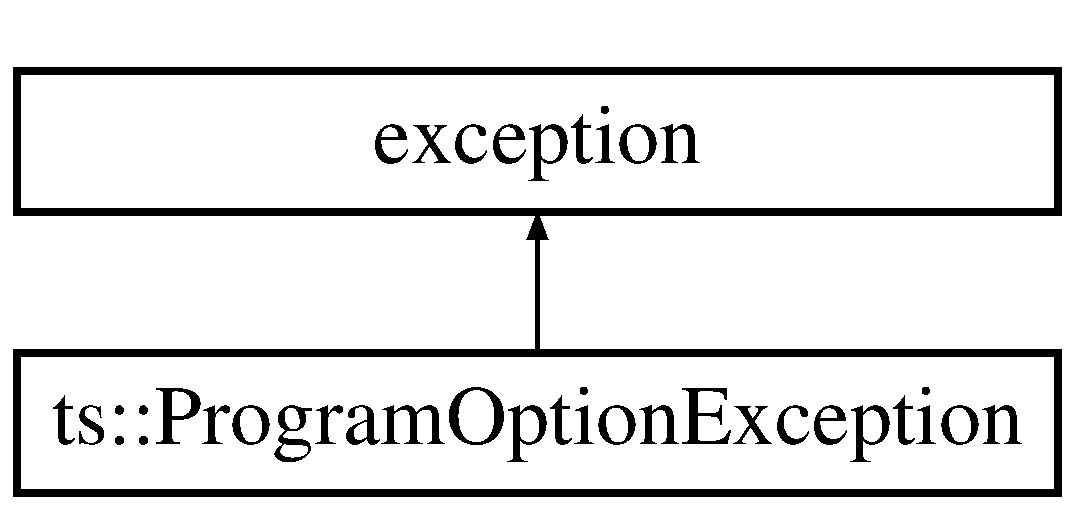
\includegraphics[height=2.000000cm]{classts_1_1_program_option_exception}
\end{center}
\end{figure}
\subsection*{Public Member Functions}
\begin{DoxyCompactItemize}
\item 
\mbox{\Hypertarget{classts_1_1_program_option_exception_ac6907eecf1de5d6f3987a6d88b623e51}\label{classts_1_1_program_option_exception_ac6907eecf1de5d6f3987a6d88b623e51}} 
{\bfseries Program\+Option\+Exception} (std\+::string const \&msg)
\item 
\mbox{\Hypertarget{classts_1_1_program_option_exception_a88bd1d294f107dfb5c8696cd7f7c3e4c}\label{classts_1_1_program_option_exception_a88bd1d294f107dfb5c8696cd7f7c3e4c}} 
virtual const char $\ast$ {\bfseries what} () const  throw ()
\end{DoxyCompactItemize}


The documentation for this class was generated from the following file\+:\begin{DoxyCompactItemize}
\item 
Program\+Option/Program\+Option\+Exception.\+hpp\end{DoxyCompactItemize}

\hypertarget{structts_1_1common_1_1_request}{}\section{ts\+:\+:common\+:\+:Request Struct Reference}
\label{structts_1_1common_1_1_request}\index{ts\+::common\+::\+Request@{ts\+::common\+::\+Request}}
Inheritance diagram for ts\+:\+:common\+:\+:Request\+:\begin{figure}[H]
\begin{center}
\leavevmode
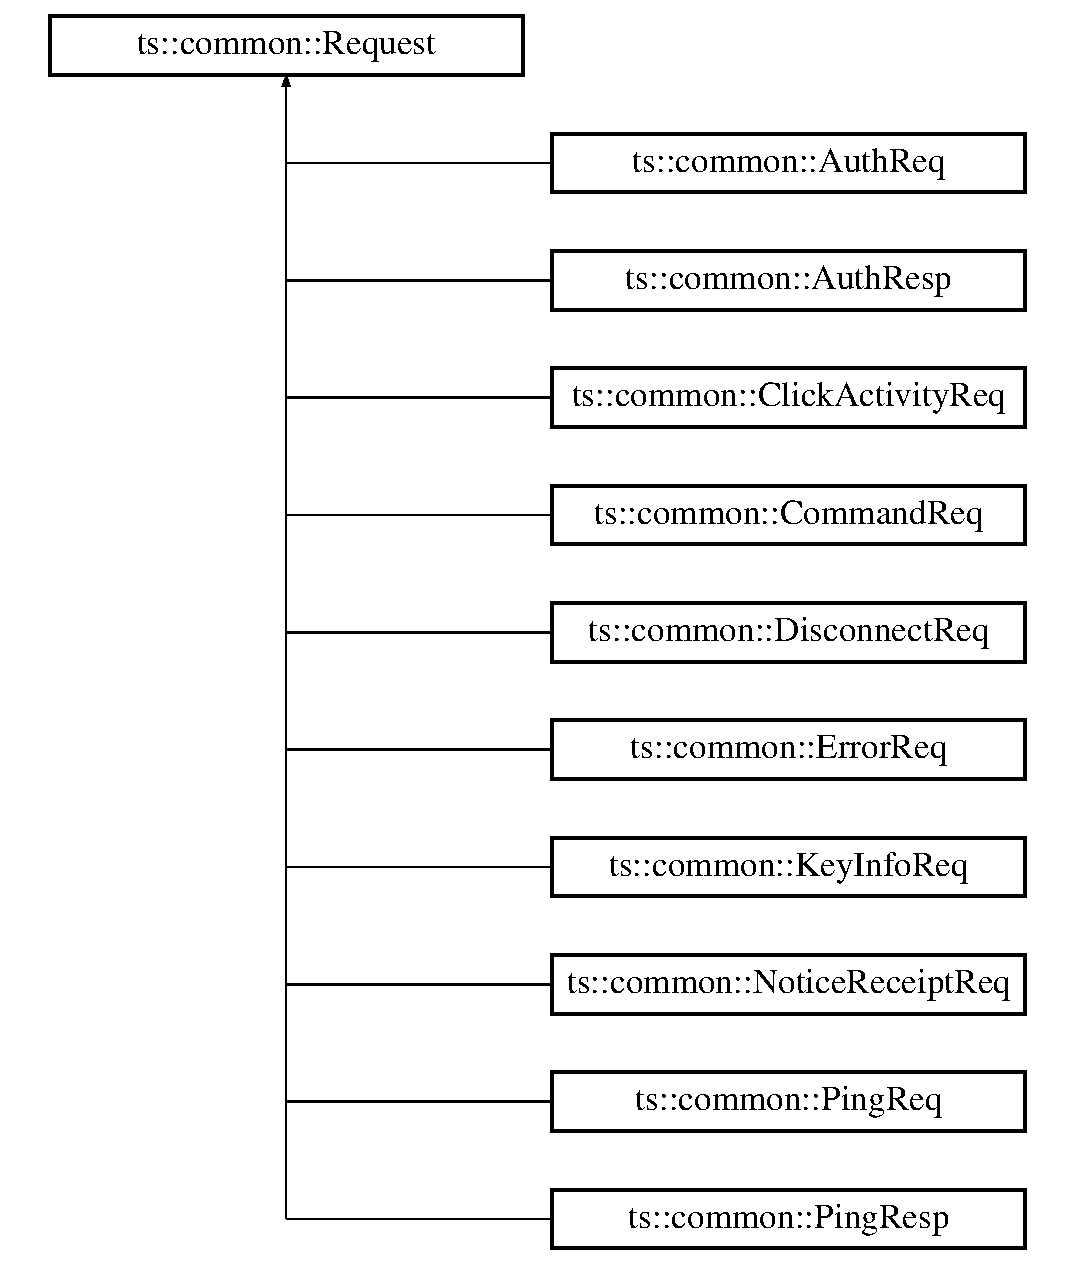
\includegraphics[height=11.000000cm]{structts_1_1common_1_1_request}
\end{center}
\end{figure}
\subsection*{Public Member Functions}
\begin{DoxyCompactItemize}
\item 
\mbox{\Hypertarget{structts_1_1common_1_1_request_adc39e5105b8968fad562455f0c1cd8dc}\label{structts_1_1common_1_1_request_adc39e5105b8968fad562455f0c1cd8dc}} 
virtual int {\bfseries get\+Id} () const =0
\item 
\mbox{\Hypertarget{structts_1_1common_1_1_request_ae001c883e781956e056ce7ea1ad0059a}\label{structts_1_1common_1_1_request_ae001c883e781956e056ce7ea1ad0059a}} 
virtual void {\bfseries from\+Json} (std\+::string const \&json)
\item 
\mbox{\Hypertarget{structts_1_1common_1_1_request_acd1c4afcfd91063a01ea181c05e6031e}\label{structts_1_1common_1_1_request_acd1c4afcfd91063a01ea181c05e6031e}} 
virtual std\+::string {\bfseries to\+Json} ()
\end{DoxyCompactItemize}
\subsection*{Public Attributes}
\begin{DoxyCompactItemize}
\item 
\mbox{\Hypertarget{structts_1_1common_1_1_request_a1f578f8c9142bf98dfeefc4e16947cf6}\label{structts_1_1common_1_1_request_a1f578f8c9142bf98dfeefc4e16947cf6}} 
std\+::string {\bfseries from}
\item 
\mbox{\Hypertarget{structts_1_1common_1_1_request_ae5c1db68c87705e6b6d86c86a581bf4a}\label{structts_1_1common_1_1_request_ae5c1db68c87705e6b6d86c86a581bf4a}} 
std\+::string {\bfseries to}
\item 
\mbox{\Hypertarget{structts_1_1common_1_1_request_abce8a750f3e89ed10e6a37c0d176151c}\label{structts_1_1common_1_1_request_abce8a750f3e89ed10e6a37c0d176151c}} 
std\+::string {\bfseries timestamp}
\end{DoxyCompactItemize}
\subsection*{Protected Attributes}
\begin{DoxyCompactItemize}
\item 
\mbox{\Hypertarget{structts_1_1common_1_1_request_ac92c52f3fe2cea815e62c0f999d569bb}\label{structts_1_1common_1_1_request_ac92c52f3fe2cea815e62c0f999d569bb}} 
\hyperlink{classts_1_1common_1_1_json_parser}{common\+::\+Json\+Parser} {\bfseries m\+Json\+Parser}
\end{DoxyCompactItemize}


The documentation for this struct was generated from the following file\+:\begin{DoxyCompactItemize}
\item 
Request/Request.\+hpp\end{DoxyCompactItemize}

\hypertarget{classts_1_1_request_handler}{}\section{ts\+:\+:Request\+Handler Class Reference}
\label{classts_1_1_request_handler}\index{ts\+::\+Request\+Handler@{ts\+::\+Request\+Handler}}
\subsection*{Public Member Functions}
\begin{DoxyCompactItemize}
\item 
\mbox{\Hypertarget{classts_1_1_request_handler_a535270343f3d8f3b492173bfb0c1cdb7}\label{classts_1_1_request_handler_a535270343f3d8f3b492173bfb0c1cdb7}} 
{\bfseries Request\+Handler} (boost\+::shared\+\_\+ptr$<$ \hyperlink{classts_1_1_client}{Client} $>$ client)
\item 
\mbox{\Hypertarget{classts_1_1_request_handler_a7a2681538784f6c2ea4844d8979fc624}\label{classts_1_1_request_handler_a7a2681538784f6c2ea4844d8979fc624}} 
void {\bfseries handle} (\hyperlink{structts_1_1common_1_1_packet}{common\+::\+Packet} const \&packet)
\end{DoxyCompactItemize}


The documentation for this class was generated from the following file\+:\begin{DoxyCompactItemize}
\item 
Request/Request\+Handler.\+hpp\end{DoxyCompactItemize}

\hypertarget{classts_1_1common_1_1_request_manager}{}\section{ts\+:\+:common\+:\+:Request\+Manager Class Reference}
\label{classts_1_1common_1_1_request_manager}\index{ts\+::common\+::\+Request\+Manager@{ts\+::common\+::\+Request\+Manager}}
\subsection*{Public Member Functions}
\begin{DoxyCompactItemize}
\item 
\mbox{\Hypertarget{classts_1_1common_1_1_request_manager_ac53eace67600d9436202506a5cc69d5b}\label{classts_1_1common_1_1_request_manager_ac53eace67600d9436202506a5cc69d5b}} 
std\+::string {\bfseries decrypt} (char const $\ast$data, bool use\+Json=false)
\item 
\mbox{\Hypertarget{classts_1_1common_1_1_request_manager_aafbf56beca0f2f2ad012b6da012b8a12}\label{classts_1_1common_1_1_request_manager_aafbf56beca0f2f2ad012b6da012b8a12}} 
{\footnotesize template$<$typename T\+Request $>$ }\\T\+Request {\bfseries decrypt} (char const $\ast$data)
\item 
\mbox{\Hypertarget{classts_1_1common_1_1_request_manager_a163e44a6f4366e6fbe91683a0cc6241f}\label{classts_1_1common_1_1_request_manager_a163e44a6f4366e6fbe91683a0cc6241f}} 
std\+::string {\bfseries encrypt} (char const $\ast$data)
\item 
\mbox{\Hypertarget{classts_1_1common_1_1_request_manager_aac5356f79cf45121bad8243a51350995}\label{classts_1_1common_1_1_request_manager_aac5356f79cf45121bad8243a51350995}} 
{\footnotesize template$<$typename T\+Request , typename... T\+Args$>$ }\\std\+::pair$<$ T\+Request, std\+::string $>$ {\bfseries prepare} (T\+Args \&\&... args)
\end{DoxyCompactItemize}


The documentation for this class was generated from the following file\+:\begin{DoxyCompactItemize}
\item 
Request/Request\+Manager.\+hpp\end{DoxyCompactItemize}

\hypertarget{classts_1_1_server_network}{}\section{ts\+:\+:Server\+Network Class Reference}
\label{classts_1_1_server_network}\index{ts\+::\+Server\+Network@{ts\+::\+Server\+Network}}
\subsection*{Public Member Functions}
\begin{DoxyCompactItemize}
\item 
\mbox{\Hypertarget{classts_1_1_server_network_ada7926cb2eb2f3f18ab41053cc8a32c3}\label{classts_1_1_server_network_ada7926cb2eb2f3f18ab41053cc8a32c3}} 
{\bfseries Server\+Network} (std\+::string const \&host, unsigned short port)
\item 
\mbox{\Hypertarget{classts_1_1_server_network_a4b36b2dff596d614deb17ad73aa0af16}\label{classts_1_1_server_network_a4b36b2dff596d614deb17ad73aa0af16}} 
void \hyperlink{classts_1_1_server_network_a4b36b2dff596d614deb17ad73aa0af16}{run} ()
\begin{DoxyCompactList}\small\item\em Run the server. \end{DoxyCompactList}\item 
\mbox{\Hypertarget{classts_1_1_server_network_aa3daa3076aa7213e98ce1527ad7f8926}\label{classts_1_1_server_network_aa3daa3076aa7213e98ce1527ad7f8926}} 
void \hyperlink{classts_1_1_server_network_aa3daa3076aa7213e98ce1527ad7f8926}{stop} ()
\begin{DoxyCompactList}\small\item\em Stop the server. \end{DoxyCompactList}\item 
void \hyperlink{classts_1_1_server_network_a4b7eb1900ddcd753e95b77e4e4b08931}{send\+Command\+To\+Clients} (std\+::string const \&msg)
\item 
void \hyperlink{classts_1_1_server_network_aa615cf28d248391c13d2f1dfb97b8d1e}{set\+Data\+Recorder} (std\+::string const \&type)
\end{DoxyCompactItemize}


\subsection{Member Function Documentation}
\mbox{\Hypertarget{classts_1_1_server_network_a4b7eb1900ddcd753e95b77e4e4b08931}\label{classts_1_1_server_network_a4b7eb1900ddcd753e95b77e4e4b08931}} 
\index{ts\+::\+Server\+Network@{ts\+::\+Server\+Network}!send\+Command\+To\+Clients@{send\+Command\+To\+Clients}}
\index{send\+Command\+To\+Clients@{send\+Command\+To\+Clients}!ts\+::\+Server\+Network@{ts\+::\+Server\+Network}}
\subsubsection{\texorpdfstring{send\+Command\+To\+Clients()}{sendCommandToClients()}}
{\footnotesize\ttfamily void ts\+::\+Server\+Network\+::send\+Command\+To\+Clients (\begin{DoxyParamCaption}\item[{std\+::string const \&}]{msg }\end{DoxyParamCaption})}

Send a message to all clients 
\begin{DoxyParams}{Parameters}
{\em msg} & \\
\hline
\end{DoxyParams}
\mbox{\Hypertarget{classts_1_1_server_network_aa615cf28d248391c13d2f1dfb97b8d1e}\label{classts_1_1_server_network_aa615cf28d248391c13d2f1dfb97b8d1e}} 
\index{ts\+::\+Server\+Network@{ts\+::\+Server\+Network}!set\+Data\+Recorder@{set\+Data\+Recorder}}
\index{set\+Data\+Recorder@{set\+Data\+Recorder}!ts\+::\+Server\+Network@{ts\+::\+Server\+Network}}
\subsubsection{\texorpdfstring{set\+Data\+Recorder()}{setDataRecorder()}}
{\footnotesize\ttfamily void ts\+::\+Server\+Network\+::set\+Data\+Recorder (\begin{DoxyParamCaption}\item[{std\+::string const \&}]{type }\end{DoxyParamCaption})}

Set the data record type 
\begin{DoxyParams}{Parameters}
{\em type} & \\
\hline
\end{DoxyParams}


The documentation for this class was generated from the following file\+:\begin{DoxyCompactItemize}
\item 
Network/Server\+Network.\+hpp\end{DoxyCompactItemize}

\hypertarget{classts_1_1common_1_1tcp_1_1_server_socket}{}\section{ts\+:\+:common\+:\+:tcp\+:\+:Server\+Socket Class Reference}
\label{classts_1_1common_1_1tcp_1_1_server_socket}\index{ts\+::common\+::tcp\+::\+Server\+Socket@{ts\+::common\+::tcp\+::\+Server\+Socket}}
\subsection*{Public Member Functions}
\begin{DoxyCompactItemize}
\item 
\mbox{\Hypertarget{classts_1_1common_1_1tcp_1_1_server_socket_a7037c67db7f87b5bc1189c30a74acd10}\label{classts_1_1common_1_1tcp_1_1_server_socket_a7037c67db7f87b5bc1189c30a74acd10}} 
{\bfseries Server\+Socket} (boost\+::asio\+::io\+\_\+service \&ios)
\item 
\mbox{\Hypertarget{classts_1_1common_1_1tcp_1_1_server_socket_ac8b82e1258042540a616e93d86d90a65}\label{classts_1_1common_1_1tcp_1_1_server_socket_ac8b82e1258042540a616e93d86d90a65}} 
void {\bfseries bind} ()
\item 
\mbox{\Hypertarget{classts_1_1common_1_1tcp_1_1_server_socket_a9c14b102664ee2a4417064cf3aa5f0b2}\label{classts_1_1common_1_1tcp_1_1_server_socket_a9c14b102664ee2a4417064cf3aa5f0b2}} 
void {\bfseries bind} (unsigned short port)
\item 
\mbox{\Hypertarget{classts_1_1common_1_1tcp_1_1_server_socket_ab95c54ec9cb464b792bd35513a133259}\label{classts_1_1common_1_1tcp_1_1_server_socket_ab95c54ec9cb464b792bd35513a133259}} 
void {\bfseries bind} (std\+::string const \&host, unsigned short port)
\item 
\mbox{\Hypertarget{classts_1_1common_1_1tcp_1_1_server_socket_a7e608369b093424bcccebef30d634625}\label{classts_1_1common_1_1tcp_1_1_server_socket_a7e608369b093424bcccebef30d634625}} 
void {\bfseries enable\+Re\+Use\+Address} ()
\item 
\mbox{\Hypertarget{classts_1_1common_1_1tcp_1_1_server_socket_a97fc3130a40289d44288b65a0d291006}\label{classts_1_1common_1_1tcp_1_1_server_socket_a97fc3130a40289d44288b65a0d291006}} 
void {\bfseries listen} (int backlog=D\+E\+F\+A\+U\+L\+T\+\_\+\+B\+A\+C\+K\+L\+OG)
\item 
\mbox{\Hypertarget{classts_1_1common_1_1tcp_1_1_server_socket_a41e1715186ecb0d0f9491e96de05fa75}\label{classts_1_1common_1_1tcp_1_1_server_socket_a41e1715186ecb0d0f9491e96de05fa75}} 
void {\bfseries run} ()
\item 
void \hyperlink{classts_1_1common_1_1tcp_1_1_server_socket_a73e30878aabcc2c1f247ae868a3c1688}{stop} ()
\item 
void \hyperlink{classts_1_1common_1_1tcp_1_1_server_socket_aab226dbcb314136342551ac145c3fb92}{async\+Accept} (On\+Client\+Accepted\+Func on\+Client\+Accepted=nullptr)
\item 
boost\+::shared\+\_\+ptr$<$ \hyperlink{classts_1_1_client}{Client} $>$ \hyperlink{classts_1_1common_1_1tcp_1_1_server_socket_a08cd736bb403fddc15755c7f873ad83d}{accept} ()
\item 
void \hyperlink{classts_1_1common_1_1tcp_1_1_server_socket_a316d4bd7d6fd81ce9c1158e3619f50e3}{set\+On\+Client\+Accepted\+Callback} (On\+Client\+Accepted\+Func on\+Client\+Accepted)
\item 
\mbox{\Hypertarget{classts_1_1common_1_1tcp_1_1_server_socket_a8fe85f1af4590956e3b19acda945244a}\label{classts_1_1common_1_1tcp_1_1_server_socket_a8fe85f1af4590956e3b19acda945244a}} 
std\+::string {\bfseries get\+Info} ()
\end{DoxyCompactItemize}
\subsection*{Protected Member Functions}
\begin{DoxyCompactItemize}
\item 
void \hyperlink{classts_1_1common_1_1tcp_1_1_server_socket_a22005ac2872f0afdecf2d405885f6551}{start\+Async\+Accept} ()
\item 
boost\+::asio\+::ip\+::tcp\+::endpoint \hyperlink{classts_1_1common_1_1tcp_1_1_server_socket_a7ed4e56f413a66650611e5d590453c03}{create\+Endpoint\+From\+Address} (std\+::string const \&host, unsigned short port)
\item 
std\+::string \hyperlink{classts_1_1common_1_1tcp_1_1_server_socket_a011cd2a3dcea435b354bdd61f7d6fc68}{get\+Address} () const
\item 
\mbox{\Hypertarget{classts_1_1common_1_1tcp_1_1_server_socket_a30944a9a77feada3889f1499a876247f}\label{classts_1_1common_1_1tcp_1_1_server_socket_a30944a9a77feada3889f1499a876247f}} 
unsigned short {\bfseries get\+Port} () const
\end{DoxyCompactItemize}
\subsection*{Protected Attributes}
\begin{DoxyCompactItemize}
\item 
\mbox{\Hypertarget{classts_1_1common_1_1tcp_1_1_server_socket_aec51a3d256cba7a66e94676af16274eb}\label{classts_1_1common_1_1tcp_1_1_server_socket_aec51a3d256cba7a66e94676af16274eb}} 
boost\+::asio\+::io\+\_\+service \& {\bfseries m\+Ios}
\item 
\mbox{\Hypertarget{classts_1_1common_1_1tcp_1_1_server_socket_a13f2d4bfbca6aa875be15619e95c1e3c}\label{classts_1_1common_1_1tcp_1_1_server_socket_a13f2d4bfbca6aa875be15619e95c1e3c}} 
boost\+::asio\+::ip\+::tcp\+::acceptor {\bfseries m\+Acceptor}
\item 
\mbox{\Hypertarget{classts_1_1common_1_1tcp_1_1_server_socket_a0d9cc76b5fb45b5cc97b7383855c1454}\label{classts_1_1common_1_1tcp_1_1_server_socket_a0d9cc76b5fb45b5cc97b7383855c1454}} 
On\+Client\+Accepted\+Func {\bfseries m\+On\+Client\+Accepted}
\end{DoxyCompactItemize}


\subsection{Member Function Documentation}
\mbox{\Hypertarget{classts_1_1common_1_1tcp_1_1_server_socket_a08cd736bb403fddc15755c7f873ad83d}\label{classts_1_1common_1_1tcp_1_1_server_socket_a08cd736bb403fddc15755c7f873ad83d}} 
\index{ts\+::common\+::tcp\+::\+Server\+Socket@{ts\+::common\+::tcp\+::\+Server\+Socket}!accept@{accept}}
\index{accept@{accept}!ts\+::common\+::tcp\+::\+Server\+Socket@{ts\+::common\+::tcp\+::\+Server\+Socket}}
\subsubsection{\texorpdfstring{accept()}{accept()}}
{\footnotesize\ttfamily boost\+::shared\+\_\+ptr$<$\hyperlink{classts_1_1_client}{Client}$>$ ts\+::common\+::tcp\+::\+Server\+Socket\+::accept (\begin{DoxyParamCaption}{ }\end{DoxyParamCaption})}

Accept new client \begin{DoxyReturn}{Returns}

\end{DoxyReturn}
\mbox{\Hypertarget{classts_1_1common_1_1tcp_1_1_server_socket_aab226dbcb314136342551ac145c3fb92}\label{classts_1_1common_1_1tcp_1_1_server_socket_aab226dbcb314136342551ac145c3fb92}} 
\index{ts\+::common\+::tcp\+::\+Server\+Socket@{ts\+::common\+::tcp\+::\+Server\+Socket}!async\+Accept@{async\+Accept}}
\index{async\+Accept@{async\+Accept}!ts\+::common\+::tcp\+::\+Server\+Socket@{ts\+::common\+::tcp\+::\+Server\+Socket}}
\subsubsection{\texorpdfstring{async\+Accept()}{asyncAccept()}}
{\footnotesize\ttfamily void ts\+::common\+::tcp\+::\+Server\+Socket\+::async\+Accept (\begin{DoxyParamCaption}\item[{On\+Client\+Accepted\+Func}]{on\+Client\+Accepted = {\ttfamily nullptr} }\end{DoxyParamCaption})}

Accept new client asynchronously with a callback 
\begin{DoxyParams}{Parameters}
{\em on\+Client\+Accepted} & \\
\hline
\end{DoxyParams}
\mbox{\Hypertarget{classts_1_1common_1_1tcp_1_1_server_socket_a7ed4e56f413a66650611e5d590453c03}\label{classts_1_1common_1_1tcp_1_1_server_socket_a7ed4e56f413a66650611e5d590453c03}} 
\index{ts\+::common\+::tcp\+::\+Server\+Socket@{ts\+::common\+::tcp\+::\+Server\+Socket}!create\+Endpoint\+From\+Address@{create\+Endpoint\+From\+Address}}
\index{create\+Endpoint\+From\+Address@{create\+Endpoint\+From\+Address}!ts\+::common\+::tcp\+::\+Server\+Socket@{ts\+::common\+::tcp\+::\+Server\+Socket}}
\subsubsection{\texorpdfstring{create\+Endpoint\+From\+Address()}{createEndpointFromAddress()}}
{\footnotesize\ttfamily boost\+::asio\+::ip\+::tcp\+::endpoint ts\+::common\+::tcp\+::\+Server\+Socket\+::create\+Endpoint\+From\+Address (\begin{DoxyParamCaption}\item[{std\+::string const \&}]{host,  }\item[{unsigned short}]{port }\end{DoxyParamCaption})\hspace{0.3cm}{\ttfamily [protected]}}

Helper for create an endpoint 
\begin{DoxyParams}{Parameters}
{\em host} & \\
\hline
{\em port} & \\
\hline
\end{DoxyParams}
\begin{DoxyReturn}{Returns}

\end{DoxyReturn}
\mbox{\Hypertarget{classts_1_1common_1_1tcp_1_1_server_socket_a011cd2a3dcea435b354bdd61f7d6fc68}\label{classts_1_1common_1_1tcp_1_1_server_socket_a011cd2a3dcea435b354bdd61f7d6fc68}} 
\index{ts\+::common\+::tcp\+::\+Server\+Socket@{ts\+::common\+::tcp\+::\+Server\+Socket}!get\+Address@{get\+Address}}
\index{get\+Address@{get\+Address}!ts\+::common\+::tcp\+::\+Server\+Socket@{ts\+::common\+::tcp\+::\+Server\+Socket}}
\subsubsection{\texorpdfstring{get\+Address()}{getAddress()}}
{\footnotesize\ttfamily std\+::string ts\+::common\+::tcp\+::\+Server\+Socket\+::get\+Address (\begin{DoxyParamCaption}{ }\end{DoxyParamCaption}) const\hspace{0.3cm}{\ttfamily [protected]}}

Return the address \begin{DoxyReturn}{Returns}

\end{DoxyReturn}
\mbox{\Hypertarget{classts_1_1common_1_1tcp_1_1_server_socket_a316d4bd7d6fd81ce9c1158e3619f50e3}\label{classts_1_1common_1_1tcp_1_1_server_socket_a316d4bd7d6fd81ce9c1158e3619f50e3}} 
\index{ts\+::common\+::tcp\+::\+Server\+Socket@{ts\+::common\+::tcp\+::\+Server\+Socket}!set\+On\+Client\+Accepted\+Callback@{set\+On\+Client\+Accepted\+Callback}}
\index{set\+On\+Client\+Accepted\+Callback@{set\+On\+Client\+Accepted\+Callback}!ts\+::common\+::tcp\+::\+Server\+Socket@{ts\+::common\+::tcp\+::\+Server\+Socket}}
\subsubsection{\texorpdfstring{set\+On\+Client\+Accepted\+Callback()}{setOnClientAcceptedCallback()}}
{\footnotesize\ttfamily void ts\+::common\+::tcp\+::\+Server\+Socket\+::set\+On\+Client\+Accepted\+Callback (\begin{DoxyParamCaption}\item[{On\+Client\+Accepted\+Func}]{on\+Client\+Accepted }\end{DoxyParamCaption})}

set the callback for the async\+Accept method \begin{DoxySeeAlso}{See also}
\hyperlink{classts_1_1common_1_1tcp_1_1_server_socket_aab226dbcb314136342551ac145c3fb92}{async\+Accept} 
\end{DoxySeeAlso}

\begin{DoxyParams}{Parameters}
{\em on\+Client\+Accepted} & \\
\hline
\end{DoxyParams}
\begin{DoxyReturn}{Returns}

\end{DoxyReturn}
\mbox{\Hypertarget{classts_1_1common_1_1tcp_1_1_server_socket_a22005ac2872f0afdecf2d405885f6551}\label{classts_1_1common_1_1tcp_1_1_server_socket_a22005ac2872f0afdecf2d405885f6551}} 
\index{ts\+::common\+::tcp\+::\+Server\+Socket@{ts\+::common\+::tcp\+::\+Server\+Socket}!start\+Async\+Accept@{start\+Async\+Accept}}
\index{start\+Async\+Accept@{start\+Async\+Accept}!ts\+::common\+::tcp\+::\+Server\+Socket@{ts\+::common\+::tcp\+::\+Server\+Socket}}
\subsubsection{\texorpdfstring{start\+Async\+Accept()}{startAsyncAccept()}}
{\footnotesize\ttfamily void ts\+::common\+::tcp\+::\+Server\+Socket\+::start\+Async\+Accept (\begin{DoxyParamCaption}{ }\end{DoxyParamCaption})\hspace{0.3cm}{\ttfamily [protected]}}

Helper for callback the async\+Accept method \mbox{\Hypertarget{classts_1_1common_1_1tcp_1_1_server_socket_a73e30878aabcc2c1f247ae868a3c1688}\label{classts_1_1common_1_1tcp_1_1_server_socket_a73e30878aabcc2c1f247ae868a3c1688}} 
\index{ts\+::common\+::tcp\+::\+Server\+Socket@{ts\+::common\+::tcp\+::\+Server\+Socket}!stop@{stop}}
\index{stop@{stop}!ts\+::common\+::tcp\+::\+Server\+Socket@{ts\+::common\+::tcp\+::\+Server\+Socket}}
\subsubsection{\texorpdfstring{stop()}{stop()}}
{\footnotesize\ttfamily void ts\+::common\+::tcp\+::\+Server\+Socket\+::stop (\begin{DoxyParamCaption}{ }\end{DoxyParamCaption})}

Stop the server 

The documentation for this class was generated from the following file\+:\begin{DoxyCompactItemize}
\item 
Socket/Tcp\+Server\+Socket.\+hpp\end{DoxyCompactItemize}

\hypertarget{classts_1_1common_1_1udp_1_1_server_socket}{}\section{ts\+:\+:common\+:\+:udp\+:\+:Server\+Socket Class Reference}
\label{classts_1_1common_1_1udp_1_1_server_socket}\index{ts\+::common\+::udp\+::\+Server\+Socket@{ts\+::common\+::udp\+::\+Server\+Socket}}
Inheritance diagram for ts\+:\+:common\+:\+:udp\+:\+:Server\+Socket\+:\begin{figure}[H]
\begin{center}
\leavevmode
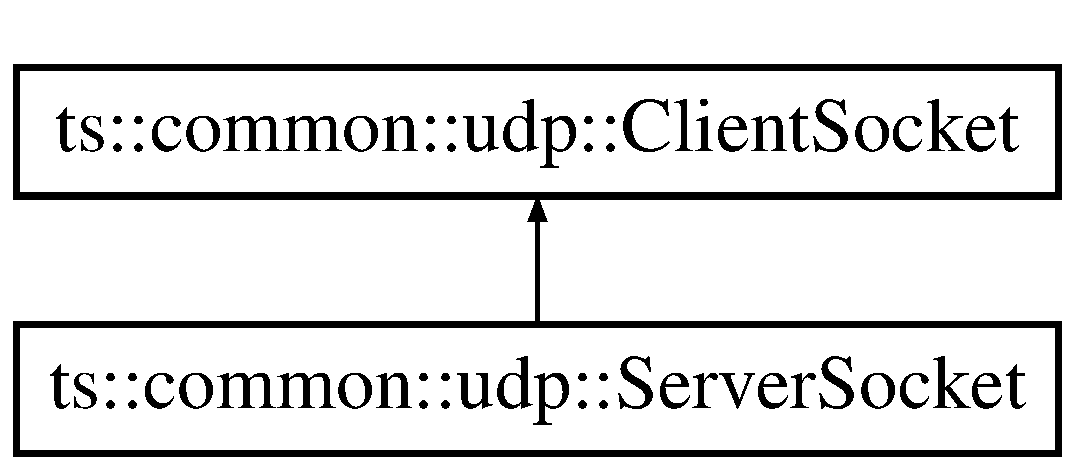
\includegraphics[height=2.000000cm]{classts_1_1common_1_1udp_1_1_server_socket}
\end{center}
\end{figure}
\subsection*{Public Member Functions}
\begin{DoxyCompactItemize}
\item 
\mbox{\Hypertarget{classts_1_1common_1_1udp_1_1_server_socket_a82b048bf21083a03578931337bd8a1d6}\label{classts_1_1common_1_1udp_1_1_server_socket_a82b048bf21083a03578931337bd8a1d6}} 
{\bfseries Server\+Socket} (boost\+::asio\+::io\+\_\+service \&ios)
\item 
\mbox{\Hypertarget{classts_1_1common_1_1udp_1_1_server_socket_a389113d153edeb689d0ce9fe66d82ae1}\label{classts_1_1common_1_1udp_1_1_server_socket_a389113d153edeb689d0ce9fe66d82ae1}} 
void {\bfseries bind} (std\+::string const \&host, unsigned short port)
\item 
\mbox{\Hypertarget{classts_1_1common_1_1udp_1_1_server_socket_ae720d8cf182cebf184a535fbb31c3d1c}\label{classts_1_1common_1_1udp_1_1_server_socket_ae720d8cf182cebf184a535fbb31c3d1c}} 
void {\bfseries run} ()
\item 
void \hyperlink{classts_1_1common_1_1udp_1_1_server_socket_a194fa6832f3ac6fa0c4b1c03abc5c8ec}{stop} ()
\end{DoxyCompactItemize}
\subsection*{Additional Inherited Members}


\subsection{Member Function Documentation}
\mbox{\Hypertarget{classts_1_1common_1_1udp_1_1_server_socket_a194fa6832f3ac6fa0c4b1c03abc5c8ec}\label{classts_1_1common_1_1udp_1_1_server_socket_a194fa6832f3ac6fa0c4b1c03abc5c8ec}} 
\index{ts\+::common\+::udp\+::\+Server\+Socket@{ts\+::common\+::udp\+::\+Server\+Socket}!stop@{stop}}
\index{stop@{stop}!ts\+::common\+::udp\+::\+Server\+Socket@{ts\+::common\+::udp\+::\+Server\+Socket}}
\subsubsection{\texorpdfstring{stop()}{stop()}}
{\footnotesize\ttfamily void ts\+::common\+::udp\+::\+Server\+Socket\+::stop (\begin{DoxyParamCaption}{ }\end{DoxyParamCaption})}

Stop the server 

The documentation for this class was generated from the following file\+:\begin{DoxyCompactItemize}
\item 
Socket/Udp\+Server\+Socket.\+hpp\end{DoxyCompactItemize}

\hypertarget{classts_1_1common_1_1_singleton}{}\section{ts\+:\+:common\+:\+:Singleton$<$ T\+Singleton $>$ Class Template Reference}
\label{classts_1_1common_1_1_singleton}\index{ts\+::common\+::\+Singleton$<$ T\+Singleton $>$@{ts\+::common\+::\+Singleton$<$ T\+Singleton $>$}}
\subsection*{Public Member Functions}
\begin{DoxyCompactItemize}
\item 
\mbox{\Hypertarget{classts_1_1common_1_1_singleton_a9fc0bee78df95f277ef75522f63ffe88}\label{classts_1_1common_1_1_singleton_a9fc0bee78df95f277ef75522f63ffe88}} 
{\bfseries Singleton} (const \hyperlink{classts_1_1common_1_1_singleton}{Singleton} \&)=delete
\item 
\mbox{\Hypertarget{classts_1_1common_1_1_singleton_aa19d30930875e015900b0223f7fcfcb6}\label{classts_1_1common_1_1_singleton_aa19d30930875e015900b0223f7fcfcb6}} 
\hyperlink{classts_1_1common_1_1_singleton}{Singleton} \& {\bfseries operator=} (const \hyperlink{classts_1_1common_1_1_singleton}{Singleton} \&)=delete
\end{DoxyCompactItemize}
\subsection*{Static Public Member Functions}
\begin{DoxyCompactItemize}
\item 
\mbox{\Hypertarget{classts_1_1common_1_1_singleton_a26a67eaeb4671b6c10fec4b3fe50645e}\label{classts_1_1common_1_1_singleton_a26a67eaeb4671b6c10fec4b3fe50645e}} 
static T\+Singleton \& {\bfseries get\+Instance} ()
\end{DoxyCompactItemize}


The documentation for this class was generated from the following file\+:\begin{DoxyCompactItemize}
\item 
Util/Singleton.\+hpp\end{DoxyCompactItemize}

\hypertarget{classts_1_1_spider_server}{}\section{ts\+:\+:Spider\+Server Class Reference}
\label{classts_1_1_spider_server}\index{ts\+::\+Spider\+Server@{ts\+::\+Spider\+Server}}
Inheritance diagram for ts\+:\+:Spider\+Server\+:\begin{figure}[H]
\begin{center}
\leavevmode
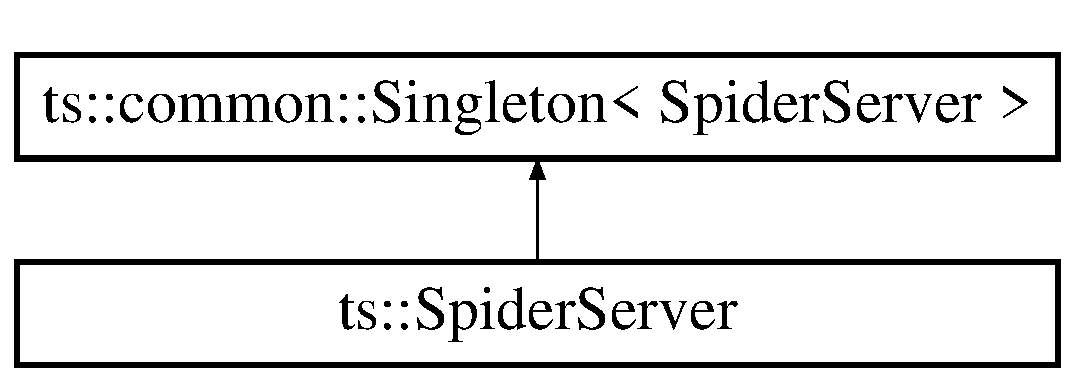
\includegraphics[height=2.000000cm]{classts_1_1_spider_server}
\end{center}
\end{figure}
\subsection*{Public Member Functions}
\begin{DoxyCompactItemize}
\item 
\mbox{\Hypertarget{classts_1_1_spider_server_afbcf37b3da1c79cb5062d8ef914cbada}\label{classts_1_1_spider_server_afbcf37b3da1c79cb5062d8ef914cbada}} 
void \hyperlink{classts_1_1_spider_server_afbcf37b3da1c79cb5062d8ef914cbada}{run} ()
\begin{DoxyCompactList}\small\item\em Run the spider server. \end{DoxyCompactList}\item 
\mbox{\Hypertarget{classts_1_1_spider_server_a396c6f71fbca158e5710eaa4c13cf959}\label{classts_1_1_spider_server_a396c6f71fbca158e5710eaa4c13cf959}} 
void \hyperlink{classts_1_1_spider_server_a396c6f71fbca158e5710eaa4c13cf959}{quit} ()
\begin{DoxyCompactList}\small\item\em Quit the spider server. \end{DoxyCompactList}\item 
void \hyperlink{classts_1_1_spider_server_afe31d95fbbdf53ca31fd3e80fdef734d}{set\+Port} (unsigned short port)
\item 
void \hyperlink{classts_1_1_spider_server_a747cb40f25dd9c9d0f6819d27647904e}{set\+File\+Path} (std\+::string const \&file\+Path)
\item 
void \hyperlink{classts_1_1_spider_server_a41cb70d329d84fbb37199556ca5e1fea}{set\+Record\+Type} (std\+::string const \&record\+Type)
\item 
void \hyperlink{classts_1_1_spider_server_a241af3e9ae7a627184b37a4b657c4ef1}{set\+Host} (std\+::string const \&host)
\item 
std\+::string \hyperlink{classts_1_1_spider_server_ac5b16b49dfd465073e0cb235b1812b6e}{get\+Info} ()
\end{DoxyCompactItemize}
\subsection*{Additional Inherited Members}


\subsection{Member Function Documentation}
\mbox{\Hypertarget{classts_1_1_spider_server_ac5b16b49dfd465073e0cb235b1812b6e}\label{classts_1_1_spider_server_ac5b16b49dfd465073e0cb235b1812b6e}} 
\index{ts\+::\+Spider\+Server@{ts\+::\+Spider\+Server}!get\+Info@{get\+Info}}
\index{get\+Info@{get\+Info}!ts\+::\+Spider\+Server@{ts\+::\+Spider\+Server}}
\subsubsection{\texorpdfstring{get\+Info()}{getInfo()}}
{\footnotesize\ttfamily std\+::string ts\+::\+Spider\+Server\+::get\+Info (\begin{DoxyParamCaption}{ }\end{DoxyParamCaption})}

Return info about the spider server \begin{DoxyReturn}{Returns}

\end{DoxyReturn}
\mbox{\Hypertarget{classts_1_1_spider_server_a747cb40f25dd9c9d0f6819d27647904e}\label{classts_1_1_spider_server_a747cb40f25dd9c9d0f6819d27647904e}} 
\index{ts\+::\+Spider\+Server@{ts\+::\+Spider\+Server}!set\+File\+Path@{set\+File\+Path}}
\index{set\+File\+Path@{set\+File\+Path}!ts\+::\+Spider\+Server@{ts\+::\+Spider\+Server}}
\subsubsection{\texorpdfstring{set\+File\+Path()}{setFilePath()}}
{\footnotesize\ttfamily void ts\+::\+Spider\+Server\+::set\+File\+Path (\begin{DoxyParamCaption}\item[{std\+::string const \&}]{file\+Path }\end{DoxyParamCaption})}

Set the file path for the data recording 
\begin{DoxyParams}{Parameters}
{\em file\+Path} & \\
\hline
\end{DoxyParams}
\mbox{\Hypertarget{classts_1_1_spider_server_a241af3e9ae7a627184b37a4b657c4ef1}\label{classts_1_1_spider_server_a241af3e9ae7a627184b37a4b657c4ef1}} 
\index{ts\+::\+Spider\+Server@{ts\+::\+Spider\+Server}!set\+Host@{set\+Host}}
\index{set\+Host@{set\+Host}!ts\+::\+Spider\+Server@{ts\+::\+Spider\+Server}}
\subsubsection{\texorpdfstring{set\+Host()}{setHost()}}
{\footnotesize\ttfamily void ts\+::\+Spider\+Server\+::set\+Host (\begin{DoxyParamCaption}\item[{std\+::string const \&}]{host }\end{DoxyParamCaption})}

Set the host 
\begin{DoxyParams}{Parameters}
{\em host} & \\
\hline
\end{DoxyParams}
\mbox{\Hypertarget{classts_1_1_spider_server_afe31d95fbbdf53ca31fd3e80fdef734d}\label{classts_1_1_spider_server_afe31d95fbbdf53ca31fd3e80fdef734d}} 
\index{ts\+::\+Spider\+Server@{ts\+::\+Spider\+Server}!set\+Port@{set\+Port}}
\index{set\+Port@{set\+Port}!ts\+::\+Spider\+Server@{ts\+::\+Spider\+Server}}
\subsubsection{\texorpdfstring{set\+Port()}{setPort()}}
{\footnotesize\ttfamily void ts\+::\+Spider\+Server\+::set\+Port (\begin{DoxyParamCaption}\item[{unsigned short}]{port }\end{DoxyParamCaption})}

Set the port 
\begin{DoxyParams}{Parameters}
{\em port} & \\
\hline
\end{DoxyParams}
\mbox{\Hypertarget{classts_1_1_spider_server_a41cb70d329d84fbb37199556ca5e1fea}\label{classts_1_1_spider_server_a41cb70d329d84fbb37199556ca5e1fea}} 
\index{ts\+::\+Spider\+Server@{ts\+::\+Spider\+Server}!set\+Record\+Type@{set\+Record\+Type}}
\index{set\+Record\+Type@{set\+Record\+Type}!ts\+::\+Spider\+Server@{ts\+::\+Spider\+Server}}
\subsubsection{\texorpdfstring{set\+Record\+Type()}{setRecordType()}}
{\footnotesize\ttfamily void ts\+::\+Spider\+Server\+::set\+Record\+Type (\begin{DoxyParamCaption}\item[{std\+::string const \&}]{record\+Type }\end{DoxyParamCaption})}

Set the type of data recording 
\begin{DoxyParams}{Parameters}
{\em record\+Type} & \\
\hline
\end{DoxyParams}


The documentation for this class was generated from the following file\+:\begin{DoxyCompactItemize}
\item 
Spider\+Server.\+hpp\end{DoxyCompactItemize}

\hypertarget{classts_1_1_sqlite_data_recorder}{}\section{ts\+:\+:Sqlite\+Data\+Recorder Class Reference}
\label{classts_1_1_sqlite_data_recorder}\index{ts\+::\+Sqlite\+Data\+Recorder@{ts\+::\+Sqlite\+Data\+Recorder}}
Inheritance diagram for ts\+:\+:Sqlite\+Data\+Recorder\+:\begin{figure}[H]
\begin{center}
\leavevmode
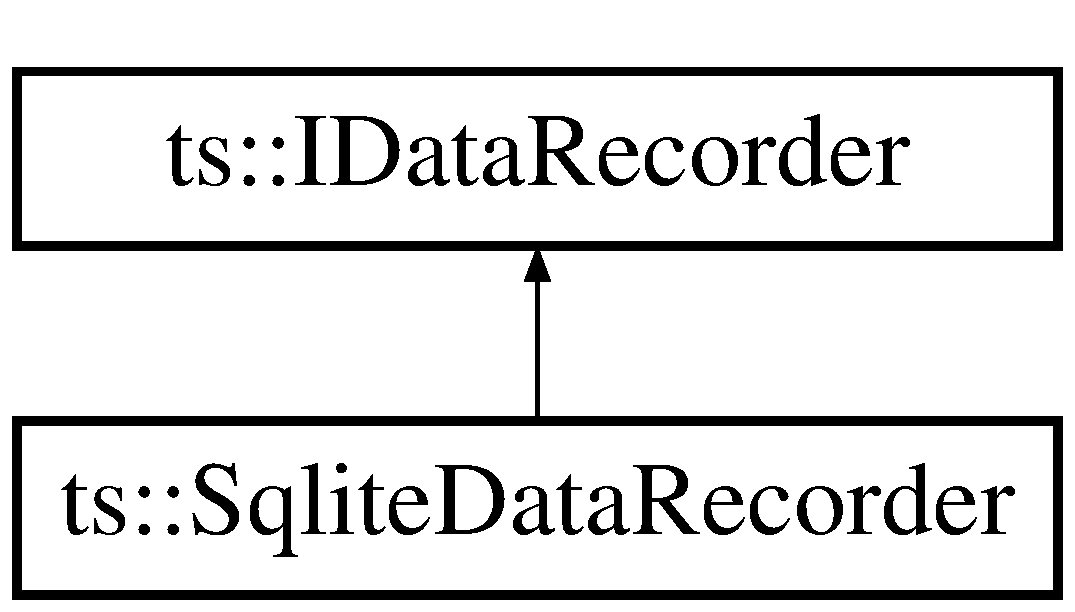
\includegraphics[height=2.000000cm]{classts_1_1_sqlite_data_recorder}
\end{center}
\end{figure}
\subsection*{Public Member Functions}
\begin{DoxyCompactItemize}
\item 
\mbox{\Hypertarget{classts_1_1_sqlite_data_recorder_a924730c2e5d94f237f58c0040297bc8b}\label{classts_1_1_sqlite_data_recorder_a924730c2e5d94f237f58c0040297bc8b}} 
void {\bfseries save} (\hyperlink{structts_1_1common_1_1_request}{common\+::\+Request} \&request) override
\end{DoxyCompactItemize}


The documentation for this class was generated from the following file\+:\begin{DoxyCompactItemize}
\item 
Data\+Recorder/Sqlite\+Data\+Recorder.\+hpp\end{DoxyCompactItemize}

%--- End generated contents ---

% Index
\backmatter
\newpage
\phantomsection
\clearemptydoublepage
\addcontentsline{toc}{chapter}{Index}
\printindex

\end{document}
